\documentclass[journal,12pt,twocolumn]{IEEEtran}
%
\usepackage{setspace}
\usepackage{gensymb}
%\doublespacing
\singlespacing

%\usepackage{graphicx}
%\usepackage{amssymb}
%\usepackage{relsize}
\usepackage[cmex10]{amsmath}
%\usepackage{amsthm}
%\interdisplaylinepenalty=2500
%\savesymbol{iint}
%\usepackage{txfonts}
%\restoresymbol{TXF}{iint}
%\usepackage{wasysym}
\usepackage{amsthm}
\usepackage{iithtlc}
\usepackage{mathrsfs}
\usepackage{txfonts}
\usepackage{stfloats}
\usepackage{bm}
\usepackage{cite}
\usepackage{cases}
\usepackage{subfig}
%\usepackage{xtab}
\usepackage{longtable}
\usepackage{multirow}
%\usepackage{algorithm}
%\usepackage{algpseudocode}
\usepackage{enumitem}
\usepackage{mathtools}
\usepackage{tikz}
\usepackage{circuitikz}
\usepackage{verbatim}
\usepackage{tfrupee}
\usepackage[breaklinks=true]{hyperref}
%\usepackage{stmaryrd}
\usepackage{tkz-euclide} % loads  TikZ and tkz-base
\usetkzobj{all}
\usepackage{listings}
    \usepackage{color}                                            %%
    \usepackage{array}                                            %%
    \usepackage{longtable}                                        %%
    \usepackage{calc}                                             %%
    \usepackage{multirow}                                         %%
    \usepackage{hhline}                                           %%
    \usepackage{ifthen}                                           %%
  %optionally (for landscape tables embedded in another document): %%
    \usepackage{lscape}     
\usepackage{multicol}
\usepackage{chngcntr}
%\usepackage{enumerate}

%\usepackage{wasysym}
%\newcounter{MYtempeqncnt}
\DeclareMathOperator*{\Res}{Res}
%\renewcommand{\baselinestretch}{2}
\renewcommand\thesection{\arabic{section}}
\renewcommand\thesubsection{\thesection.\arabic{subsection}}
\renewcommand\thesubsubsection{\thesubsection.\arabic{subsubsection}}

\renewcommand\thesectiondis{\arabic{section}}
\renewcommand\thesubsectiondis{\thesectiondis.\arabic{subsection}}
\renewcommand\thesubsubsectiondis{\thesubsectiondis.\arabic{subsubsection}}

% correct bad hyphenation here
\hyphenation{op-tical net-works semi-conduc-tor}
\def\inputGnumericTable{}                                 %%

\lstset{
%language=C,
frame=single, 
breaklines=true,
columns=fullflexible
}
%\lstset{
%language=tex,
%frame=single, 
%breaklines=true
%}

\begin{document}
%


\newtheorem{theorem}{Theorem}[section]
\newtheorem{problem}{Problem}
\newtheorem{proposition}{Proposition}[section]
\newtheorem{lemma}{Lemma}[section]
\newtheorem{corollary}[theorem]{Corollary}
\newtheorem{example}{Example}[section]
\newtheorem{definition}[problem]{Definition}
%\newtheorem{thm}{Theorem}[section] 
%\newtheorem{defn}[thm]{Definition}
%\newtheorem{algorithm}{Algorithm}[section]
%\newtheorem{cor}{Corollary}
\newcommand{\BEQA}{\begin{eqnarray}}
\newcommand{\EEQA}{\end{eqnarray}}
\newcommand{\define}{\stackrel{\triangle}{=}}

\bibliographystyle{IEEEtran}
%\bibliographystyle{ieeetr}


\providecommand{\mbf}{\mathbf}
\providecommand{\pr}[1]{\ensuremath{\Pr\left(#1\right)}}
\providecommand{\qfunc}[1]{\ensuremath{Q\left(#1\right)}}
\providecommand{\sbrak}[1]{\ensuremath{{}\left[#1\right]}}
\providecommand{\lsbrak}[1]{\ensuremath{{}\left[#1\right.}}
\providecommand{\rsbrak}[1]{\ensuremath{{}\left.#1\right]}}
\providecommand{\brak}[1]{\ensuremath{\left(#1\right)}}
\providecommand{\lbrak}[1]{\ensuremath{\left(#1\right.}}
\providecommand{\rbrak}[1]{\ensuremath{\left.#1\right)}}
\providecommand{\cbrak}[1]{\ensuremath{\left\{#1\right\}}}
\providecommand{\lcbrak}[1]{\ensuremath{\left\{#1\right.}}
\providecommand{\rcbrak}[1]{\ensuremath{\left.#1\right\}}}
\theoremstyle{remark}
\newtheorem{rem}{Remark}
\newcommand{\sgn}{\mathop{\mathrm{sgn}}}
\providecommand{\abs}[1]{\left\vert#1\right\vert}
\providecommand{\res}[1]{\Res\displaylimits_{#1}} 
\providecommand{\norm}[1]{\left\lVert#1\right\rVert}
%\providecommand{\norm}[1]{\lVert#1\rVert}
\providecommand{\mtx}[1]{\mathbf{#1}}
\providecommand{\mean}[1]{E\left[ #1 \right]}
\providecommand{\fourier}{\overset{\mathcal{F}}{ \rightleftharpoons}}
%\providecommand{\hilbert}{\overset{\mathcal{H}}{ \rightleftharpoons}}
\providecommand{\system}{\overset{\mathcal{H}}{ \longleftrightarrow}}
	%\newcommand{\solution}[2]{\textbf{Solution:}{#1}}
\newcommand{\solution}{\noindent \textbf{Solution: }}
\newcommand{\cosec}{\,\text{cosec}\,}
\providecommand{\dec}[2]{\ensuremath{\overset{#1}{\underset{#2}{\gtrless}}}}
\newcommand{\myvec}[1]{\ensuremath{\begin{pmatrix}#1\end{pmatrix}}}
\newcommand{\mydet}[1]{\ensuremath{\begin{vmatrix}#1\end{vmatrix}}}
%\numberwithin{equation}{section}
%\numberwithin{equation}{subsection}
%\numberwithin{problem}{section}
%\numberwithin{definition}{section}
\makeatletter
\@addtoreset{figure}{problem}
\makeatother

\let\StandardTheFigure\thefigure
\let\vec\mathbf
%\renewcommand{\thefigure}{\theproblem.\arabic{figure}}
\renewcommand{\thefigure}{\theproblem}
%\setlist[enumerate,1]{before=\renewcommand\theequation{\theenumi.\arabic{equation}}
%\counterwithin{equation}{enumi}


%\renewcommand{\theequation}{\arabic{subsection}.\arabic{equation}}

\def\putbox#1#2#3{\makebox[0in][l]{\makebox[#1][l]{}\raisebox{\baselineskip}[0in][0in]{\raisebox{#2}[0in][0in]{#3}}}}
     \def\rightbox#1{\makebox[0in][r]{#1}}
     \def\centbox#1{\makebox[0in]{#1}}
     \def\topbox#1{\raisebox{-\baselineskip}[0in][0in]{#1}}
     \def\midbox#1{\raisebox{-0.5\baselineskip}[0in][0in]{#1}}

\vspace{3cm}

\title{
	\logo{
Optimization through School Geometry
	}
}
\author{ G V V Sharma$^{*}$% <-this % stops a space
	\thanks{*The author is with the Department
		of Electrical Engineering, Indian Institute of Technology, Hyderabad
		502285 India e-mail:  gadepall@iith.ac.in. All content in this manual is released under GNU GPL.  Free and open source.}
	
}	
%\title{
%	\logo{Matrix Analysis through Octave}{\begin{center}
\includegraphics[scale=.24]{tlc}\end{center}}{}{HAMDSP}
%}


% paper title
% can use linebreaks \\ within to get better formatting as desired
%\title{Matrix Analysis through Octave}
%
%
% author names and IEEE memberships
% note positions of commas and nonbreaking spaces ( ~ ) LaTeX will not break
% a structure at a ~ so this keeps an author's name from being broken across
% two lines.
% use \thanks{} to gain access to the first footnote area
% a separate \thanks must be used for each paragraph as LaTeX2e's \thanks
% was not built to handle multiple paragraphs
%

%\author{<-this % stops a space
%\thanks{}}
%}
% note the % following the last \IEEEmembership and also \thanks - 
% these prevent an unwanted space from occurring between the last author name
% and the end of the author line. i.e., if you had this:
% 
% \author{....lastname \thanks{...} \thanks{...} }
%                     ^------------^------------^----Do not want these spaces!
%
% a space would be appended to the last name and could cause every name on that
% line to be shifted left slightly. This is one of those "LaTeX things". For
% instance, "\textbf{A} \textbf{B}" will typeset as "A B" not "AB". To get
% "AB" then you have to do: "\textbf{A}\textbf{B}"
% \thanks is no different in this regard, so shield the last } of each \thanks
% that ends a line with a % and do not let a space in before the next \thanks.
% Spaces after \IEEEmembership other than the last one are OK (and needed) as
% you are supposed to have spaces between the names. For what it is worth,
% this is a minor point as most people would not even notice if the said evil
% space somehow managed to creep in.



% The paper headers
%\markboth{Journal of \LaTeX\ Class Files,~Vol.~6, No.~1, January~2007}%
%{Shell \MakeLowercase{\textit{et al.}}: Bare Demo of IEEEtran.cls for Journals}
% The only time the second header will appear is for the odd numbered pages
% after the title page when using the twoside option.
% 
% *** Note that you probably will NOT want to include the author's ***
% *** name in the headers of peer review papers.                   ***
% You can use \ifCLASSOPTIONpeerreview for conditional compilation here if
% you desire.




% If you want to put a publisher's ID mark on the page you can do it like
% this:
%\IEEEpubid{0000--0000/00\$00.00~\copyright~2007 IEEE}
% Remember, if you use this you must call \IEEEpubidadjcol in the second
% column for its text to clear the IEEEpubid mark.



% make the title area
\maketitle

\newpage

\tableofcontents

\bigskip

\renewcommand{\thefigure}{\theenumi}
\renewcommand{\thetable}{\theenumi}
%\renewcommand{\theequation}{\theenumi}

%\begin{abstract}
%%\boldmath
%In this letter, an algorithm for evaluating the exact analytical bit error rate  (BER)  for the piecewise linear (PL) combiner for  multiple relays is presented. Previous results were available only for upto three relays. The algorithm is unique in the sense that  the actual mathematical expressions, that are prohibitively large, need not be explicitly obtained. The diversity gain due to multiple relays is shown through plots of the analytical BER, well supported by simulations. 
%
%\end{abstract}
% IEEEtran.cls defaults to using nonbold math in the Abstract.
% This preserves the distinction between vectors and scalars. However,
% if the journal you are submitting to favors bold math in the abstract,
% then you can use LaTeX's standard command \boldmath at the very start
% of the abstract to achieve this. Many IEEE journals frown on math
% in the abstract anyway.

% Note that keywords are not normally used for peerreview papers.
%\begin{IEEEkeywords}
%Cooperative diversity, decode and forward, piecewise linear
%\end{IEEEkeywords}



% For peer review papers, you can put extra information on the cover
% page as needed:
% \ifCLASSOPTIONpeerreview
% \begin{center} \bfseries EDICS Category: 3-BBND \end{center}
% \fi
%
% For peerreview papers, this IEEEtran command inserts a page break and
% creates the second title. It will be ignored for other modes.
%\IEEEpeerreviewmaketitle

\begin{abstract}
This manual shows how to balance chemical equations using matrices.
%book provides an introduction to optimization  based on the NCERT textbooks from Class 6-12.  Links to sample Python codes are available in the text.  
\end{abstract}
Download python codes using 
\begin{lstlisting}
svn co https://github.com/gadepall/school/trunk/training/chemistry/codes
\end{lstlisting}

%\section{Problem}
Balance the following chemical equation
%
\begin{align}
\label{eq:chem_balance}
Fe+H_2O &\rightarrow Fe_3O_4 + H_2
\end{align}
%
\solution Let the balanced version of \eqref{eq:chem_balance} be 
%the coefficients for each compound be
%
\begin{align}
x_1Fe+x_2H_2 O &\rightarrow x_3Fe_3 O_4 + x_4H_2
\end{align}
%
which results in the following equations
%
\begin{align}
\begin{split}
\brak{x_1 -3x_3}Fe &= 0
\\
\brak{2x_2 -2x_4}H &= 0
\\
\brak{x_2 -4x_3}H &= 0
\end{split}
\\
\implies 
\begin{split}
x_1 -3x_3 &= 0
\\
2x_2 -2x_4 &= 0
\\
x_2 -4x_3 &= 0
\end{split}
\end{align}
%
resulting in the matrix equation
\begin{align}
\label{eq:chem_balance_mat_eq}
\begin{split}
\myvec{
1 & 0 & -3 & 0
\\
0 & 2 & 0 & -2
\\
0 & 1 & -4 & 0
}
\vec{x} &= \vec{0}
\end{split}
\end{align}
%
where
\begin{align}
\vec{x} = \myvec{x_1 \\ x_2 \\ x_3 \\ x_4} 
\end{align}
The matrix in \eqref{eq:chem_balance_mat_eq} can be row reduced as follows
%
\begin{align}
\label{eq:chem_balance_mat_eq}
\myvec{
1 & 0 & -3 & 0
\\
0 & 2 & 0 & -2
\\
0 & 1 & -4 & 0
}
 \xleftrightarrow[]{R_2 \leftarrow \frac{R_2}{2}}
\myvec{
1 & 0 & -3 & 0
\\
0 & 1 & 0 & -1
\\
0 & 1 & -4 & 0
}
\\
 \xleftrightarrow[]{R_3\leftarrow R_3-R_2}
\myvec{
1 & 0 & -3 & 0
\\
0 & 1 & 0 & -1
\\
0 & 0 & -4 & 1
}
 \xleftrightarrow[]{R_1\leftarrow 4R_1-3R_3}
\myvec{
-4 & 0 & 0 & -3
\\
0 & 1 & 0 & -1
\\
0 & 0 & -4 & 1
}
\\
 \xleftrightarrow[R_3 \leftarrow -\frac{1}{4}R_3]{R_1\leftarrow -\frac{1}{4}}
\myvec{
1 & 0 & 0 & \frac{3}{4}
\\
0 & 1 & 0 & -1
\\
0 & 0 & 1 & \frac{1}{4}
}
\end{align}
%
Thus, 
\begin{align}
\vec{x} = x_4\myvec{\frac{3}{4} \\ -1 \\ \frac{1}{4} \\ 1}
\end{align}

%\section{Triangle}
%\subsection{Triangle Examples}
%\renewcommand{\theequation}{\theenumi}
\begin{enumerate}[label=\arabic*.,ref=\thesubsection.\theenumi]
\numberwithin{equation}{enumi}
%
\item Do the points $\vec{A}=\myvec{3\\2}, \vec{B}=\myvec{-2\\-3}, \vec{C}=\myvec{2\\3} $ form a triangle?  If so, name the type of triangle formed.
\label{prob:tri_exam_coll_pts}
%
\\
\solution The direction vectors of $AB$ and $BC$ are 
\begin{align}
\label{eq:tri_geo_ex_baorth}
\vec{B}-\vec{A} &= \myvec{-5\\-5}
\\
\vec{C}-\vec{A} &= \myvec{-1\\1}
\label{eq:tri_geo_ex_caorth}
\end{align}
%
Since 
%
\begin{align}
\vec{B}-\vec{A} \ne k\brak{\vec{C}-\vec{A}},
\end{align}
%
the points are not collinear and form a triangle.  An alternative method is to create the matrix
\begin{align}
\label{eq:tri_geo_ex_diff_mat}
\vec{M} = \myvec{\vec{B}-\vec{A} & \vec{B}-\vec{A}}^T 
\end{align}
%
If $rank(\vec{M}) = 1$, the points are collinear.  The rank of a matrix is the number of nonzero rows left after doing row operations.  In this problem, 
%
\begin{align}
\vec{M} = \myvec{-5 & -5\\-1 & 1}\xleftrightarrow {R_2\leftarrow 5R_2-R_1}\myvec{-5 & -5\\0 & 10}
\\
\implies rank(\vec{M}) = 2
\end{align}
%
as the number of non zero rows is 2.
The following code plots Fig. \ref{fig:check_tri}
%
\begin{lstlisting}
codes/triangle/check_tri.py
\end{lstlisting}
%
\begin{figure}[!ht]
\includegraphics[width=\columnwidth]{./triangle/figs/check_tri.eps}
\caption{}
\label{fig:check_tri}
\end{figure}
%
From the figure, it appears that $\triangle ABC$ is right angled, with $BC$ as the hypotenuse.  From Baudhayana's theorem, this would be true if 
\begin{align}
\norm{\vec{B}-\vec{A}}^2+\norm{\vec{C}-\vec{A}}^2&=\norm{\vec{B}-\vec{C}}^2
\end{align}
which, from \eqref{eq:tri_const_norm_ac} can be expressed as
\begin{multline}
\norm{\vec{A}}^2 + \norm{\vec{C}}^2 - 2\vec{A}^T\vec{C}+
\norm{\vec{A}}^2 + \norm{\vec{B}}^2 - 2\vec{A}^T\vec{B}
\\
=
\norm{\vec{B}}^2 + \norm{\vec{C}}^2 - 2\vec{B}^T\vec{C}
\end{multline}
%
to obtain 
\begin{align}
\label{eq:tri_geo_ex_orth}
\brak{\vec{B}-\vec{A}}^T\brak{\vec{C}-\vec{A}}&=0
\end{align}
%
after simplification.  From \eqref{eq:tri_geo_ex_baorth} and \eqref{eq:tri_geo_ex_caorth}, it is easy to verify that 
\begin{align}
\label{eq:tri_geo_ex_orth_sol}
\brak{\vec{B}-\vec{A}}^T\brak{\vec{C}-\vec{A}}=
 \myvec{-5 & -5}\myvec{-1\\1} = 0
\end{align}
satisfying
\eqref{eq:tri_geo_ex_orth}. Thus,  $\triangle ABC$ is right angled at $\vec{A}$.
%
\item Find the area of a triangle whose vertices are 
$\vec{A}=\myvec{1\\-1}, 
\vec{B} = \myvec{-4\\6}$ and
$ 
\vec{C} = \myvec{-3\\-5}
$.
%
\\
\solution In Fig. \ref{fig:rt_triangle}, from Baudhayana's theorem, 
\begin{align}
\label{eq:tri_geo_baudh}
b^2 = a^2+c^2 &
\\
=b^2\cos^2C+b^2\sin^2C &
\\
\implies \cos^2C+\sin^2C &= 1
\end{align}
%
In Fig. \ref{fig:tri_const_ex_cos_form}, the area of $\triangle ABC$ is defined as
{\footnotesize
\begin{align}
\label{eq:tri_geo_area_sin_form}
\frac{1}{2}ah &= \frac{1}{2}ab\sin C
\\
&=\frac{1}{2}ab\sqrt{1-\cos^2C} \quad \brak{\text{from } \eqref{eq:tri_geo_baudh}
}
\\
&=\frac{1}{2}ab\sqrt{1-\brak{\frac{a^2+b^2-c^2}{2ab}}^2} \brak{\text{from } \eqref{eq:cosC}
}
\\
&=\frac{1}{4}\sqrt{\brak{2ab}^2-\brak{a^2+b^2-c^2}}
\\
&=\frac{1}{4}\sqrt{\brak{2ab+a^2+b^2-c^2}\brak{2ab-a^2-b^2+c^2}}
\\
&= \frac{1}{4}\sqrt{\cbrak{\brak{a+b}^2-c^2}\cbrak{c^2-\brak{a-b}^2}}
\\
&= \frac{1}{4}\sqrt{\brak{a+b+c}\brak{a+b-c}\brak{a+c-b}\brak{b+c-a}}
\label{eq:tri_ex_hero_temp}
\end{align}
}
Substituting 
%
\begin{align}
s=\frac{a+b+c}{2}
\end{align}
%
in \eqref{eq:tri_ex_hero_temp}, the area of $\triangle ABC$ is 
%
\begin{align}
\sqrt{s\brak{s-a}\brak{s-b}\brak{s-c}}
\end{align}
%
This is known as Hero's formula.  The following code computes the area of the  triangle as 24.
%
\begin{lstlisting}
codes/triangle/area_tri.py
\end{lstlisting}
%
%
\item Find the area of a triangle formed by the vertices $\vec{A}=\myvec{5\\2}, \vec{B}=\myvec{4\\7}, \vec{C}=\myvec{7\\-4}$.
\\
\solution  The area of $\triangle ABC$ is also obtained  in terms of the  {\em magnitude} of the determinant of the matrix $\vec{M}$ in  \eqref{eq:tri_geo_ex_diff_mat} as
%
\begin{align}
\frac{1}{2}\mydet{\vec{M}}
\end{align}
The computation is done in \textbf{area\_tri.py}
\item Find the area of a triangle formed by the points $\vec{P}=\myvec{-1.5\\3}, \vec{Q}=\myvec{6\\-2}, \vec{R}=\myvec{-3\\4}$.
\\
\solution Another formula for the area of $\triangle ABC$  is
%
\begin{align}
\frac{1}{2}\mydet{1 & 1 & 1\\ \vec{A} & \vec{B} & \vec{C} }
\end{align}
%
\item Find the area of a triangle having the points
%
\begin{align}
\vec{A} = \myvec{1\\1 \\1},
\vec{B} = \myvec{1\\2 \\3},
\vec{C} = \myvec{2\\ 3\\1}
\end{align}
%
as its vertices.
\\
\solution The area of a triangle using the {\em vector product} is obtained as
\begin{align}
\frac{1}{2}\norm{\brak{\vec{B}-\vec{A}}\times \brak{\vec{C}-\vec{A}}}
\end{align}
%
For any two vectors $\vec{a}=\myvec{a_1\\a_2\\a_3}, \vec{b}=\myvec{b_1\\b_2\\b_3}$, 
\begin{align}
\label{eq:tri_cross_prod}
\vec{a}\times \vec{b} = \myvec{0 & -a_3 & a_2 \\ a_3 & 0 & -a_1 \\ -a_2 & a_1 & 0}\myvec{b_1\\b_2\\b_3}
\end{align}
%
The following code computes the area using the vector product.
%
\begin{lstlisting}
codes/triangle/area_tri_vec.py
\end{lstlisting}
%
%
\item The centroid of a $\triangle ABC$ is at the point \myvec{1\\1\\1}.  If the coordinates of $\vec{A}$ and $\vec{B}$ are \myvec{3\\-5\\7} and \myvec{-1\\7\\-6}, respectively, find the coordinates of the point $\vec{C}$.
%
\\
\solution The centroid of $\triangle ABC$ is given by
\begin{align}
\label{eq:tri_geo_ex_centroid}
\vec{O} = \frac{\vec{A}+\vec{B}+\vec{C}}{3}
\end{align}
%
Thus, 
\begin{align}
\vec{C} = 3\vec{C}-\vec{A}-\vec{B}
\end{align}
%
\item Show that the points 
\begin{align}
\vec{A} = \myvec{2\\-1 \\1},
\vec{B} = \myvec{1\\-3 \\-5},
\vec{C} = \myvec{3\\ -4\\-4}
\end{align}
%
are the vertices of a right angled triangle.
\\
\solution 
The following code plots Fig. \ref{fig:triangle_3d}
%
\begin{lstlisting}
codes/triangle/triangle_3d.py
\end{lstlisting}
%
\begin{figure}[!ht]
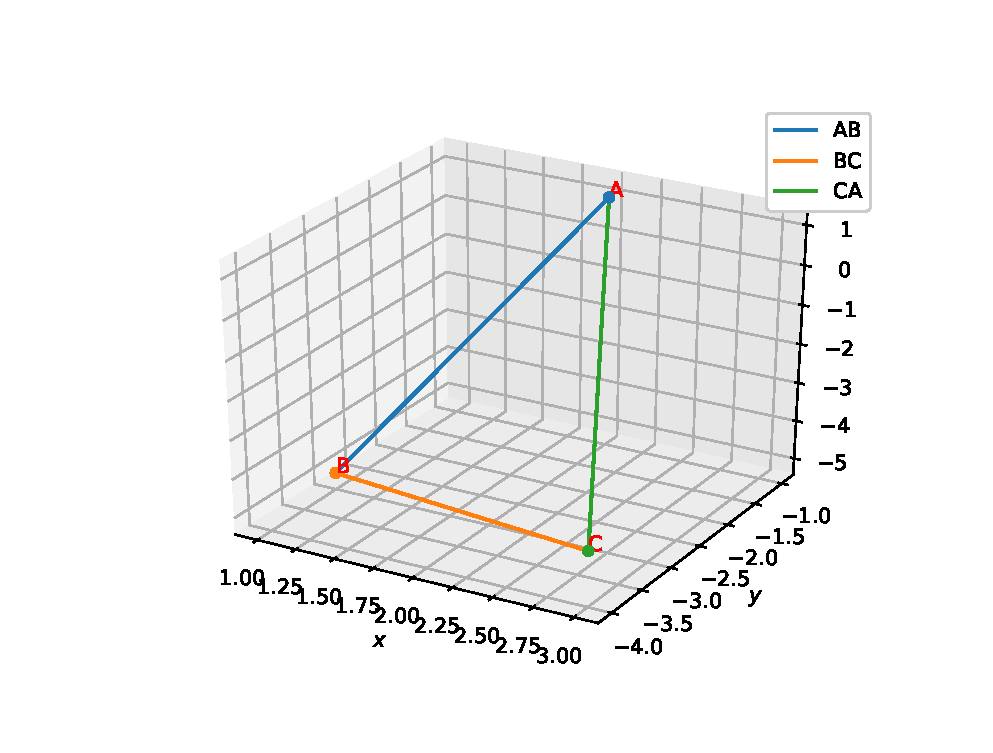
\includegraphics[width=\columnwidth]{./triangle/figs/triangle_3d.eps}
\caption{}
\label{fig:triangle_3d}
\end{figure}
%
From the figure, it appears that $\triangle ABC$ is right angled at $\vec{C}$.  Since 
\begin{align}
\brak{\vec{A}-\vec{C}}^T\brak{\vec{B}-\vec{C}}&=0
\end{align}
%
it is proved that the triangle is indeed right angled.
 \item Are the points 
\begin{align}
\vec{A} = \myvec{3\\6 \\9},
\vec{B} = \myvec{10\\20 \\30},
\vec{C} = \myvec{25\\ -41\\5},
\end{align}
%
the vertices of a right angled triangle?
%
\item A tower stands vertically on the ground.  From a point on the ground, which is 15m away from the foot of the tower, the angle of elevation of the top of the tower is found to be 60$\degree$.  Find the height of the tower.
%
\begin{figure}[!ht]
\includegraphics[width=\columnwidth]{./triangle/figs/Trig/pg1.eps}
\caption{}
\label{fig:trig_pg1}
\end{figure}
%
\\
\solution Fig. \ref{fig:trig_pg1} summarizes the problem. 
%
\begin{align}
h = b\tan\theta = 15\tan60\degree = 15\sqrt{3}
\end{align}
%
\item An electrician has to repair an electric fault pole of height 5m.  She needs to reach a point 1.3m below the top of the pole to undertake the repair work.  What should be the length of the ladder that she should use which, when inclined at an angle of 60$\degree$ to the horizontal, would enable her to reach the required position?  Also, how far from the foot of the pole should she place the foot of the ladder?
%
\begin{figure}[!ht]
\includegraphics[width=\columnwidth]{./triangle/figs/Trig/pg2.eps}
\caption{}
\label{fig:trig_pg2}
\end{figure}
%
\\
\solution Fig. \ref{fig:trig_pg2} summarizes the problem. The objective is to find $l$ and $b$.  From the figure,
%
if 
\begin{align}
\cot \theta &=\frac{1}{\tan \theta},
\\
h-x &= l\sin \theta = b\tan \theta
\\
\implies l &= \brak{h-x}\csc \theta = 3.7\csc60\degree 
\\
\text{and } b&=\brak{h-x}\cot\theta = 3.7 \cot \degree 
\end{align}
\item An observer 1.5m tall is 28.5m away from a chimney.  The angle of elevation of the top of the chimney from her eyes is 45$\degree$.  What is the height of the chimney?
%
%
\begin{figure}[!ht]
\includegraphics[width=\columnwidth]{./triangle/figs/Trig/pg3.eps}
\caption{}
\label{fig:trig_pg3}
\end{figure}
%
\\
\solution Fig. \ref{fig:trig_pg3} summarizes the problem. The objective is to find $h$.  From the figure,
%
\begin{align}
h-h_1 &=  b\tan \theta
\\
\implies h &= h_1+b\tan\theta 
\\
&= 1.5+28.5\tan45\degree 
\\
&= 30m
\end{align}
\item From a point $\vec{P}$ on the ground the angle of elevation of the top of a 10m tall building is 30$\degree$.  A flag is hoisted at the top of the building and the angle of elevation of the top of the flagstaff from $\vec{P}$ is $45\degree$.  Find the length of the flagstaff and the distance of the building from the point $\vec{P}$.
%
\begin{figure}[!ht]
\includegraphics[width=\columnwidth]{./triangle/figs/Trig/pg4.eps}
\caption{}
\label{fig:trig_pg4}
\end{figure}
%
\\
\solution Fig. \ref{fig:trig_pg4} summarizes the problem. The objective is to find $h_2$ and $b$ while $h_1$ is known.  From the figure, 
%
\begin{align}
h_1+h_2 &=  b\tan \theta_1
\\
h_1 &= b\tan \theta_2
\end{align}
%
This can be expressed as the matrix equation 
%
\begin{align}
\myvec{
\tan \theta_1 & -1
\\
\tan \theta_2 &0
}\myvec{b\\h_2}
= h_1\myvec{1\\1}
\end{align}
%
and solved.
\item The shadow of a tower standing on a level ground is found to be 40m longer when the Sun's altitude is 30$\degree$ than when it is $60\degree$.  Find the height of the tower.
%
\begin{figure}[!ht]
\includegraphics[width=\columnwidth]{./triangle/figs/Trig/pg5.eps}
\caption{}
\label{fig:trig_pg5}
\end{figure}
%
\\
\solution Fig. \ref{fig:trig_pg5} summarizes the problem. The objective is to find $h$.  from the figure,
%
\begin{align}
b_1 &= h\cot 60\degree
\\
b_2 &= h\cot 30\degree
\\
b_2-b_1 &= 40
\\
\implies h \brak{\cot 30\degree-\cot 60\degree}&= 40
\\
\text{or } h &= \frac{40}{\cot 30\degree-\cot 60\degree}
\end{align}
%
\item The angles of depression of the top and the bottom of an 8m tall building from the top of a multi-storeyed building are 30$\degree$ and 45$\degree$ respectively.  Find the height of the multi-storeyed building and the distance between the two buildings.
%
\begin{figure}[!ht]
\includegraphics[width=\columnwidth]{./triangle/figs/Trig/pg6.eps}
\caption{}
\label{fig:trig_pg6}
\end{figure}
%
\\
\solution Fig. \ref{fig:trig_pg6} summarizes the problem. The objective is to find $h_2$ and $b$.  From the figure, 
%
\begin{align}
h_2 &= b\tan \theta_2
\\
h_2-h_1 &= b\tan \theta_1
\end{align}
%
which can be expressed as
%
\begin{align}
\myvec{
 1 & -\tan\theta_2 
\\
 1 & -\tan\theta_1
}\myvec{h_2\\b}
= h_1\myvec{0\\1}
\end{align}
%
and solved.
\end{enumerate}
%
 
%\subsection{Triangle Exercises}
%\renewcommand{\theequation}{\theenumi}
\begin{enumerate}[label=\arabic*.,ref=\thesubsection.\theenumi]
\numberwithin{equation}{enumi}
%
\item Draw the graphs of the equations 
\begin{align}
\myvec{1 & -1}\vec{x} + 1 &= 0 
\\
\myvec{ 3 & 2} - 12 &= 0
\end{align}
%
 Determine the coordinates of the vertices of the triangle formed by these lines and the x-axis, and shade the triangular region.
%
\item The vertices of $\triangle PQR$ are 

$
\vec{P} = \myvec{2 \\1},
\vec{Q} = \myvec{-2\\3},
\vec{R} = \myvec{4\\5}.
$
Find the equation of the median through the vertex $\vec{R}$.
\item In the $\triangle ABC$ with vertices
$
\vec{A}=\myvec{2\\3}, 
\vec{B}=\myvec{4\\-1},
 \vec{C}=\myvec{1\\2}
$,
find the equation and length of the altitude from the vertex $\vec{A}$.
\item Find the area of the triangle whose vertices are
\begin{enumerate}
\item \myvec{2\\3}, \myvec{-1\\0},  \myvec{2\\-4}
\item  \myvec{-5\\-1},  \myvec{3\\-5},  \myvec{5\\2}
\end{enumerate}
\item Find the area of the triangle formed by joining the mid points o the sides of a triangle whose vertices are  \myvec{0\\-1},  \myvec{2\\1},  \myvec{0\\3}.
\item Verify that the median of $\triangle ABC$ with vertices $\vec{A}=\myvec{4\\-6},  \vec{B}=\myvec{3\\-2}$ and  $\vec{C} =  \myvec{5\\2}$ divides it into two triangles of equal areas.
\item The vertices of $\triangle ABC$ are $\vec{A}=\myvec{4\\6},  \vec{B}=\myvec{1\\5}$ and  $\vec{C} =  \myvec{7\\2}$.  A line is drawn to intersect sides $AB$ and $AC$ at $D$ and $E$ respectively, such that
\begin{align}
\frac{AD}{AB}=\frac{AE}{AC}= \frac{1}{4}
\end{align}
%
Find 
\begin{align}
\frac{\text{area of }\triangle ADE}{\text{area of }\triangle ABC}.
\end{align}
\item Let $\vec{A}=\myvec{4\\2},  \vec{B}=\myvec{6\\5}$ and  $\vec{C} =  \myvec{1\\4}$ be the vertices of $\triangle ABC$.
\begin{enumerate}
\item The median from $\vec{A}$ meets $BC$ at $\vec{D}$.  Find the coordinates of the point $\vec{D}$.
\item Find the coordinates of the point $\vec{P}$ on $AD$ such that $AP:PD = 2:1$.
\item Find the coordinates of the points $\vec{Q}$ and $\vec{R}$ on medians $BE$ and $CF$ respectively such that $BQ:QE = 2:1$ and $CR:RF = 2:1$.
\end{enumerate}
\item In $\triangle ABC$, Show that the centroid 
\begin{align}
\vec{O} = \frac{\vec{A}+\vec{B}+\vec{C}}{3}
\end{align}
\item Show that the points 
\begin{align}
\vec{A} = \myvec{2\\-1 \\1},
\vec{B} = \myvec{1\\-3 \\-5},
\vec{C} = \myvec{3\\ -4\\-4}
\end{align}
%
are the vertices of a right angled triangle.
\item In $\triangle ABC$, 
$
\vec{A} = \myvec{1\\2 \\3},
\vec{B} = \myvec{-1\\0 \\0},
\vec{C} = \myvec{0\\ 1\\2}.
$
Find $\angle B$.
\item Show that the vectors 
$
\myvec{2\\-1 \\1},
\myvec{1\\-3 \\-5},
\myvec{3\\ -4\\-4}
$
form the vertices of a right angled triangle.
\item Find the area of a triangle having the points 
$
\vec{A} = \myvec{1\\1 \\1},
\vec{B} = \myvec{1\\2 \\3}, \text{ and }
\vec{C} = \myvec{2\\ 3\\1}
$
as its vertices.
\item Find the area of a triangle with vertices
$
\vec{A} = \myvec{1\\1 \\2},
\vec{B} = \myvec{2\\3 \\5}, \text{ and }
\vec{C} = \myvec{1\\ 5\\5}
$
\item A girl walks 4km west, then she walks 3km in a direction $30\degree$ east of north and stops.  Determine the girl's displacement from her initial point of departure.
\item Find the direction vectors of the sides of a triangle with vertices
$
\vec{A} = \myvec{3\\5 \\-4},
\vec{B} = \myvec{-1\\1 \\2}, \text{ and }
\vec{C} = \myvec{-5\\ -5\\-2}
$
\item Without using the Pythagoras theorem, show that the points \myvec{4\\ 4}, \myvec{3\\ 5} and \myvec{–1\\ –1} are the vertices of a right angled triangle.
\item Check whether 
\begin{align}
\myvec{5\\-2}, \myvec{6\\4}, \myvec{7\\-2}
\end{align}
are the vertices of an isosceles triangle.
%
\item A circus artist is climbing a 20m long rope, which is tightly stretched and tied from the top of a vertical pole to the ground.  Find the height of the pole, if the angle made by the rope with the ground level is 30$\degree$.
%
\item A tree breaks due to storm and the broken part bends so that the top of the tree touches the ground making an angle of 30$\degree$ with it.  The distance between the foot of the tree to the point where the top touches the ground is 8m.  Find the height of the tree.
%
\item A contractor plans to install two slides for the children to play in a park.  For the children below the age of 5 years, she prefers to have a slide whose top is at a height of 1.5m, and is inclined at an angle of 30$\degree$  to the ground, whereas for elder children she wants to have a steep slide at a height of 3m, and inclined at an angle of 60$\degree$ to the ground.  What should be the length of the slide in each case?
%
\item The angle of elevation of the top of a tower from a point on the ground, which is 30m away from the foot of the tower, is 30$\degree$.  Find the height of the tower.
%
\item A kite is flying at a height of 60m above the ground.  The string attached to the kite is temporarily tied to a point on the ground.  The inclination of the string with the ground is $60\degree$.  Find the length of the string, assuming that there is no slack in the string.
%
\item A 1.5m tall boy is standing at some distance from a 30m tall building.  The angle of elevation from his eyes to the top of the building increases from 30$\degree$
 to 60$\degree $ as he walks towards the building.  Find the distance he walked towards the building.

\item From a point on the ground, the angles of elevation of the bottom and the top of a transmission tower fixed at the top of a 20 m high building are 45$\degree$ and 60$\degree$ respectively. Find the height of the tower.

\item A statue, 1.6 m tall, stands on the top of a pedestal. From a point on the ground, the angle of elevation of the top of the statue is 60$\degree$ and from the same point the angle of elevation of the top of the pedestal is 45$\degree$. Find the height of the pedestal.
\item The angle of elevation of the top of a building from the foot of the tower is 30$\degree$ and the angle of elevation of the top of the tower from the foot of the building is 60$\degree$. If the tower is 50 m high, find the height of the building.
\item Two poles of equal heights are standing opposite each other on either side of the road, which is 80 m wide. From a point between them on the road, the angles of elevation of the top of the poles are 60$\degree$ and 30$\degree$, respectively. Find the height of the poles and the distances of the point from the poles.
\item A TV tower stands vertically on a bank of a canal. From a point on the other bank directly opposite the tower, the angle of elevation of the top of the tower is 60$\degree$. From another point 20 m away from this point on the line joing this point to the foot of the tower, the angle of elevation of the top of the tower is 30$\degree$. Find the height of the tower and the width of the canal.
\item From the top of a 7 m high building, the angle of elevation of the top of a cable tower is 60$\degree$ and the angle of depression of its foot is 45$\degree$. Determine the height of the tower.
\item As observed from the top of a 75 m high lighthouse from the sea-level, the angles of depression of two ships are 30$\degree$ and 45$\degree$. If one ship is exactly behind the other on the same side of the lighthouse, find the distance between the two ships.
\item A 1.2 m tall girl spots a balloon moving with the wind in a horizontal line at a height of 88.2 m from the ground. The angle of elevation of the balloon from the eyes of the girl at any instant is 60$\degree$. After some time, the angle of elevation reduces to 30$\degree$. Find the distance travelled by the balloon during the interval.
\item A straight highway leads to the foot of a tower. A man standing at the top of the tower observes a car at an angle of depression of 30$\degree$, which is approaching the foot of the tower with a uniform speed. Six seconds later, the angle of depression of the car is found to be 60$\degree$. Find the time taken by the car to reach the foot of the tower from this point.
\item The angles of elevation of the top of a tower from two points at a distance of 4 m and 9 m from the base of the tower and in the same straight line with it are complementary. Prove that the height of the tower is 6 m.

\end{enumerate}
%

 
%%
%\section{Quadrilateral}
%\subsection{Quadrilateral Examples}
%\renewcommand{\theequation}{\theenumi}
\begin{enumerate}[label=\arabic*.,ref=\thesubsection.\theenumi]
\numberwithin{equation}{enumi}
%
\item Sum of the angles of a quadrilateral is 360$\degree$. 
\\
\solution Draw the diagonal and use the fact that sum of the angles of a triangle is 180$\degree$.
\item  A diagonal of a parallelogram divides it into two congruent triangles. 
\\
\solution The alternate angles for the parallel sides are equal.  The diagonal is common.  Use ASA congruence.
%
\item  In a parallelogram, 
\begin{enumerate}
\item opposite sides are equal 
\item  opposite angles are equal
\item  diagonals bisect each other
\end{enumerate}
%
\solution Since the diagonal divides the parallelogram into two congruent triangles, all the above results follow.
%
\item  A quadrilateral is a parallelogram, if 
%
\begin{enumerate}
\item opposite sides are equal or 
\item  opposite angles are equal or 
\item  diagonals bisect each other or 
\item a pair of opposite sides is equal and parallel
\end{enumerate}
%
\solution All the above lead to a quadrilateral that has two parallel sides, by showing that the alternate angles are equal.
%
%
\item A rectangle is a parallelogram with one angle that is 90$\degree$.  Show that all angles of the rectangle are 90$\degree$.
%
\\
\solution Draw a diagonal.  Since the diagonal divides the rectangle into two congruent triangles, the angle opposite to the right angle is also 90$\degree$. Using congruence, it can be shown that the other two angles are equal.  Now use the fact that the sum of the angles of a quadrilateral is 360$\degree$.
%
\item  Diagonals of a rectangle bisect each other and are equal and vice-versa. 
%
\\
\solution Use Baudhayana's theorem for equality of diagonals.
%
\item  Diagonals of a rhombus bisect each other at right angles and vice-versa. 
%
\\
\solution The median of an isoceles triangle is also its perpendicular bisector.
%
\item  Diagonals of a square bisect each other at right angles and are equal, and vice-versa. 
%
\\
\solution A square has the properties of a rectangle as well as a rhombus.
%
\item  The line-segment joining the mid-points of any two sides of a triangle is parallel to the third side and is half of it.
\label{prob:quad_similar}
%
\\
\solution If $DE$ is the lie joining he mid points of $\triangle ABC$,  use cosine formula to find the lengths of $DE$ and $BC$. Then use cosine formula to show that all angles of $\triangle ADE$ are equal to the corresponding angles of $\triangle ABC$.
%
\item  A line through the mid-point of a side of a triangle parallel to another side bisects the third side.
\\
\solution Use cosine formula.
%
\item  The quadrilateral formed by joining the mid-points of the sides of a quadrilateral, in order, is a parallelogram.
%
\\
\solution Draw one diagonal and use Problem \eqref{prob:quad_similar}.  Repeat for the other diagonal to show that the sides are parallel.
%
\item Two parallel lines l and m are intersected by a transversal p. Show that the quadrilateral formed by the bisectors of interior angles is a rectangle.
%
\item Show that the bisectors of angles of a parallelogram form a rectangle.
%
\item A quadrilateral is a parallelogram if a pair of opposite sides is equal and parallel.
%
\item $ABCD$ is a parallelogram in which $P$ and $Q$ are mid-points of opposite sides $AB$ and $CD$. If $AQ$ intersects $DP$ at $S$ and $BQ$ intersects $CP$ at $R$, show that: 
%
\begin{enumerate}
\item  $APCQ$ is a parallelogram. 
\item $DPBQ$ is a parallelogram. 
\item $PSQR$ is a parallelogram.
\end{enumerate}
%
\item In $\triangle ABC, D, E$ and $F$ are respectively the mid-points of sides $AB, BC$ and $CA $. Show that $\triangle ABC$ is divided into four congruent triangles by joining $D, E$ and $F$.
\item $l, m$ and $n$ are three parallel lines intersected by transversals $p$ and $q$ such that $l, m$ and $n$ cut off equal intercepts $AB$ and $BC$ on $p$ . Show that $l, m$ and $n$ cut off equal intercepts $DE$ and $EF$ on $q$ also.
%

\item Show that the points $\vec{A} = \myvec{1\\7}, \vec{B} = \myvec{4\\2}, \vec{C}=\myvec{-1\\-1},\vec{D}= \myvec{-4\\4} $  are the vertices of a square.
\\
\solution By inspection, 
%
\begin{align}
\frac{\vec{A}+\vec{C}}{2}=\frac{\vec{B}+\vec{D}}{2} = \myvec{0\\3}
\end{align}
%
Hence, the diagonals $AC$ and $BD$ bisect each other.
%
Also, 
\begin{align}
\brak{\vec{A}-\vec{C}}^T
\brak{\vec{B}-\vec{D}} = 0
\end{align}
%
$\implies AC \perp BD $.  Hence $ABCD$ is a square.
\item If the points
$
\vec{A} = \myvec{6\\1}, 
\vec{B} = \myvec{8\\2}, 
\vec{C} = \myvec{9\\4}, 
\vec{D} = \myvec{p\\3}
$
are the vertices of a parallelogram, taken in order, find the value of $p$.
\\
\solution In the parallelogram $ABCD$, $AC$ and $BD$ bisect each other.  This can be used to find $p$.
\item If $\vec{A} = \myvec{-5\\7}, \vec{B} = \myvec{-4\\-5}, \vec{C} = \myvec{-1\\-6}, \vec{D} = \myvec{4\\5}$, find the area of the quadrilateral $ABCD$.
%
\\
\solution The area of  $ABCD$ is the sum of the areas of trianges ABD and CBD and is given by 
\begin{multline}
\frac{1}{2}\norm{\brak{\vec{A}-\vec{B}}\times \brak{\vec{A}-\vec{D}}}
\\
+
\frac{1}{2}\norm{\brak{\vec{C}-\vec{B}}\times \brak{\vec{C}-\vec{D}}}
\end{multline}
\item Show that the points 
$\vec{A} = \myvec{1\\2\\3},
 \vec{B} = \myvec{-1\\-2\\-1},
\vec{C} = \myvec{2\\3\\2},
\vec{D} = \myvec{4\\7\\6}.
$
are the vertices of a parallelogram $ABCD$ but it is not a rectangle.
%
\\
\solution Since the direction vectors
%
\begin{align}
\vec{A}-\vec{B}&= \vec{D}-\vec{C}
\\
\vec{A}-\vec{D}&= \vec{B}-\vec{C}
\end{align}
%
$AB \parallel CD$ and $AD \parallel BC$.  Hence $ABCD$ is a parallelogram.  However, 
%
\begin{align}
\brak{\vec{A}-\vec{B}}^T\brak{ \vec{A}-\vec{D}}\ne 0
\end{align}
%
Hence, it is not a rectangle.
The following code plots Fig. \ref{fig:quad_3d}
%
\begin{lstlisting}
codes/triangle/quad_3d.py
\end{lstlisting}
%
\begin{figure}[!ht]
\includegraphics[width=\columnwidth]{./triangle/figs/quad_3d.eps}
\caption{}
\label{fig:quad_3d}
\end{figure}
%

\item Find the area of a parallelogram whose adjacent sides are given by the vectors \myvec{3\\1\\4} and \myvec{1\\-1\\1}.
%
\\
\solution  The area is given by 
%
\begin{align}
\frac{1}{2}\norm{\myvec{3\\1\\4} \times \myvec{1\\-1\\1}}
\end{align}
%
\item Kamla has a triangular field with sides 240 m, 200 m, 360 m, where she grew wheat. In another triangular field with sides 240 m, 320 m, 400 m adjacent to the previous field, she wanted to grow potatoes and onions. She divided the field in two parts by joining the mid-point of the longest side to the opposite vertex and grew patatoes in one part and onions in the other part. Draw the figure for this problem.  How much area (in hectares) has been used for wheat, potatoes and onions? (1 hectare = 10000 $m^2$).
\item Students of a school staged a rally for cleanliness campaign. They walked through the lanes in two groups. One group walked through the lanes AB, BC and CA; while the other through AC, CD and DA. Then they cleaned the area enclosed within their lanes. If AB = 9 m, BC = 40 m, CD = 15 m, DA = 28 m and $\angle B = 90\degree$, which group cleaned more area and by how much? Draw the corresponding figure.  Find the total area cleaned by the students (neglecting the width of the lanes). 
%
\item Sanya has a piece of land which is in the shape of a rhombus. She wants her one daughter and one son to work on the land and produce different crops. She divided the land in two equal parts. If the perimeter of the land is 400 m and one of the diagonals is 160 m, how much area each of them will get for their crops? Draw the rhombus.
\end{enumerate}
%
 
%\subsection{Quadrilateral Geometry}
%\renewcommand{\theequation}{\theenumi}
\begin{enumerate}[label=\arabic*.,ref=\thesubsection.\theenumi]
\numberwithin{equation}{enumi}

\item Draw a quadrilateral in the Cartesian plane, whose vertices are \myvec{– 4\\ 5}, \myvec{0\\ 7}, \myvec{5\\ – 5} and \myvec{– 4\\ –2}. Also, find its area.
\item Find the area of a rhombus if its vertices are \myvec{3\\0}, \myvec{4\\5}, \myvec{-1\\4} and \myvec{-2\\-1} taken in order.
\item Without using distance formula, show that points \myvec{– 2\\ – 1}, \myvec{4\\ 0}, \myvec{3\\ 3} and \myvec{–3\\ 2} are the vertices of a parallelogram.
\item  Find the area of the quadrilateral whose vertices, taken in order, are 
 \myvec{-4\\2},  \myvec{-3\\-5},  \myvec{3\\-2},  \myvec{2\\3}. 
\item The two opposite vertices of a square are \myvec{-1\\2},  \myvec{3\\2}. Find the coordinates of the other two vertices.
\item $ABCD$ is a rectangle formed by the points $\vec{A} = \myvec{-1\\-1}, \vec{B} = \myvec{-1\\4}, \vec{C} = \myvec{5\\4}, \vec{D} = \myvec{5\\-1}$. $ \vec{P}, \vec{Q}, \vec{R}, \vec{S}$ are the mid points of $AB, BC, CD, DA$ respectively.  Is the quadrilateral $PQRS$ a 
\begin{enumerate}
\item square?
\item rectangle?
\item rhombus?
\end{enumerate}
\item Find the area of a parallelogram whose adjacent sides are given by the vectors \myvec{3\\1\\4} and \myvec{1\\-1\\1}.
\item Find the area of a parallelogram whose adjacent sides are determined by the vectors $\vec{a} = \myvec{1\\-1\\3}$ and $\vec{b}=\myvec{2\\-7\\1}$.
\item Find the area of a rectangle $ABCD$ with vertices
$\vec{A} = \myvec{-1\\\frac{1}{2}\\ 4},
 \vec{B} = \myvec{1\\\frac{1}{2}\\ 4},
\vec{C} = \myvec{1\\-\frac{1}{2}\\ 4},
\vec{D} = \myvec{-1\\-\frac{1}{2}\\ 4}.
$
\item The two adjacent sides of a parallelogram are \myvec{2\\ -4 \\ -5} and  \myvec{1\\-2\\ -3}. Find the unit vector parallel to its diagonal.  Also, find its area.
\end{enumerate}
%
 
%
%\section{Constrained Optimization}
%%\subsection{Equality Constraint}
%\renewcommand{\theequation}{\theenumi}
\begin{enumerate}[label=\arabic*.,ref=\thesubsection.\theenumi]
\numberwithin{equation}{enumi}

\item Do the points $\myvec{3\\2}, \myvec{-2\\-3}, \myvec{2\\3} $ form a triangle?  If so, name the type of triangle formed.

\item Show that the points $\myvec{1\\7}, \myvec{4\\2}, \myvec{-1\\-1}, \myvec{-4\\4} $  are the vertices of a square.
\item Verify if $\vec{A} = \myvec{3\\1}, \vec{B} = \myvec{6\\4}, \vec{C} = \myvec{8\\6}$ are points on a line.
\item Find the condition for $\vec{x} = \myvec{x_1\\x_2}$ to be equidistant from the points $\myvec{7\\1}, \myvec{3\\5}$.
\item Find a point on the $y$-axis which is equidistant from the points $\vec{A} = \myvec{6\\5}, \vec{B} = \myvec{-4\\3}$.
\item Draw a line segement of length 7.6 cm and divide it in the ratio $5:8$.
\\
\solution Let the end points of the line be 
\begin{align}
\vec{A} = \myvec{0\\0}, \vec{B} = \myvec{7.6\\0}
\end{align}
Then the point $\vec{C}$
\begin{align}
\vec{C} = \frac{k \vec{A} + \vec{B}}{k+1}
\end{align}
divides $AB$ in the ration $k:1$. For the given problem, $k = \frac{5}{8}$.
The following code plots Fig. \ref{fig:section}
\begin{lstlisting}
codes/line/draw_section.py
\end{lstlisting}
\begin{figure}[!ht]
\includegraphics[width=\columnwidth]{./line/figs/section.eps}
\caption{}
\label{fig:section}
\end{figure}
\item Find a unit vector in the  direction of \myvec{2\\3\\1}.
\item Find the direction vector of $PQ$, where 
\begin{align}
\vec{P} = \myvec{2\\3\\0},
\vec{Q} = \myvec{-1\\-2\\-4}
\end{align}
\item Find the angle between the vectors 
\begin{align}
\myvec{1\\-2\\3},
\myvec{3\\-2\\1}
\end{align}
\item Find the projection of the vector 
\begin{align}
\myvec{1\\3\\7}
\end{align}
on the vector
\begin{align}
\myvec{7\\-1\\8}
\end{align}
\item Find a unit vector perpendicular to each of the vectors
$\vec{a}+\vec{b}$ and $\vec{a}-\vec{b}$, where 
\begin{align}
\vec{a}=\myvec{1\\1\\1},
\vec{b}=\myvec{1\\2\\3}.
\end{align}
\item Write down a unit vector in the xy-plane, makeing an angle of $30\degree$ with the positive direction of the x-axis.
\item Find the value of $x$ for which $x\myvec{1\\1\\1}$ is a unit vector.
\item Find the direction vectors and slopes of the lines passing through the points
%
\begin{enumerate}
\item \myvec{3\\-2} and \myvec{-1\\4}.
\item \myvec{3\\-2} and \myvec{7\\-2}.
\item \myvec{3\\-2} and \myvec{3\\4}.
\item Making an inclination of $60\degree$ with the positive direction of the x-axis.
\end{enumerate}
%
\item If the angle between two lines is $\frac{\pi}{4}$ and the slope of one of the lines is $\frac{1}{4}$ find the slope of the other line.
\item The line through the points \myvec{-2\\6} and \myvec{4\\8} is perpendicular to the line through the points \myvec{8\\12} and $\myvec{x\\24}$.  Find the value of $x$.
\item Find the equations of the lines parallel to axes and passing through \myvec{– 2, 3}.
\item Find the equation of the line through \myvec{– 2\\ 3} with slope –4.
\item Write the equation of the line through the points \myvec{1\\-1} and \myvec{3\\5}.
\item Wrire the equation of the lines for which $\tan \theta = \frac{1}{2}$, where $\theta$ is the inclination of the line and 
\begin{enumerate}
\item y-intercept is $-\frac{3}{2}$
\item x-intercept is 4.
\end{enumerate}
\item Find the equation of the line, which makes intercepts -3 and 2 on the x and y axes respectively.
\item Find the equation of the line whose perpendicular distance from the origin is 4 units and the angle which the normal makes with the positive direction of x-axis is $15\degree$.
\item Two positions of time and distance are recorded as, when $T = 0, D = 2$ and when $T = 3, D = 8$. Using the concept of slope, find law of motion, i.e., how distance depends upon time.
\item The Farenheit temperature $F$ and absolute temperature $K$ satisfy a linear equation.  Given $K=273$ when $F=32$ and that $K=373$  when $F=212$, express $K$ in terms of $F$ and find the value of $F$, when $K=0$.
\item Equation of a line is 
\begin{align}
\myvec{3 & – 4} + 10 = 0. 
\end{align}
Find its 
\begin{enumerate}
\item  slope, 
\item  x - and y-intercepts.
\end{enumerate}
\item Find the angle between the lines 
\begin{align}
\myvec{1 & – \sqrt{3}}\vec{x}  = 5
\\
\myvec{\sqrt{3} & –1}\vec{x}  = -6
. 
\end{align}
\item Find the equation of a line perpendicular to the line 
\begin{align}
\myvec{1 & – 2}\vec{x}  = 3
\end{align}
%
and passes through the point \myvec{1\\-2}.
\item Find the distance of the point \myvec{3\\-5} from the line 
\begin{align}
\myvec{3 & – 4}\vec{x}  = 26
\end{align}
\item If the lines 
\begin{align}
\myvec{2 & 1}\vec{x}  = 3
\\
\myvec{5 & k}\vec{x}  = 3
\\
\myvec{3 & 1}\vec{x}  = 2
\end{align}
%
are concurrent, find the value of $k$.
%
\item Find the distance of the line
\begin{align}
\myvec{4 & 1}\vec{x}  = 0
\end{align}
%
from the point \myvec{4\\1} measured along the line making an angle of $135\degree$ with the positive x-axis.
\item Assuming that straight lines work as a plane mirror for a point, find the image of the point \myvec{1\\2} in the line 
%
\begin{align}
\myvec{1 & -3}\vec{x}  = -4.
\end{align}
%
\item A line is such that its segment between the lines %
\begin{align}
\myvec{5 & -1}\vec{x}  &= -4
\\
\myvec{3 & 4}\vec{x}  &= 4
\end{align}
%
is bisected at the point \myvec{1\\5}.  Obtain its equation.
%
\item Show that the path of a moving point such that its distances from two lines
%
\begin{align}
\myvec{3 & -2}\vec{x}  &= 5
\\
\myvec{3 & 2}\vec{x}  &= 5
\end{align}
%
are  equal is a straight line.
\end{enumerate}
%

%\section{Convex Function}
%\renewcommand{\theequation}{\theenumi}
%\subsection{Problem}

\begin{enumerate}[label=\arabic*.,ref=\thesection.\theenumi]
\numberwithin{equation}{enumi}

\item
The following python script plots 
%
\begin{align}
f(\lambda) = a\lambda^2 + b\lambda + d
\label{eq:parab}
\end{align}
%
for 
\begin{align}
a &= \norm{\vec{m}}^2 > 0
\\
b &= \vec{m}^T\brak{\vec{A} -\vec{P}} 
\\
c &= \norm{\vec{A} -\vec{P}}^2
\end{align}
where $\vec{A}$ is the intercept of the line $L$ in \eqref{eq:opt_line_nor}
on the x-axis and the points
\begin{align}
\vec{U} &= \myvec{\lambda_1\\f(\lambda_1)}, 
\vec{V} = \myvec{\lambda_2\\f(\lambda_2)}
\\
\vec{X} &= \myvec{t \lambda_1 + \brak{1-t}\lambda_2 \\ f\sbrak{t \lambda_1 + \brak{1-t}\lambda_2}},
\\
\vec{Y} &= \myvec{t \lambda_1 + \brak{1-t}\lambda_2 \\ t f\brak{\lambda_1} + \brak{1-t}f\brak{\lambda_2}}
\end{align}
%
for 
\begin{align}
\lambda_1 = -3, 
\lambda_2 = 4, 
t = 0.3
\end{align}
in Fig. \ref{fig:conv_def}. Geometrically, this means that any point $\vec{Y}$ between the points $\vec{U}, \vec{V}$ on the line $UV$ is always above the point $\vec{X}$ on the curve $f(\lambda)$.
Such a  function $f$ is defined to be {\em convex} function 
%
\begin{lstlisting}
codes/optimization/1.2.py
\end{lstlisting}
%
%%
\begin{figure}[!ht]
\centering
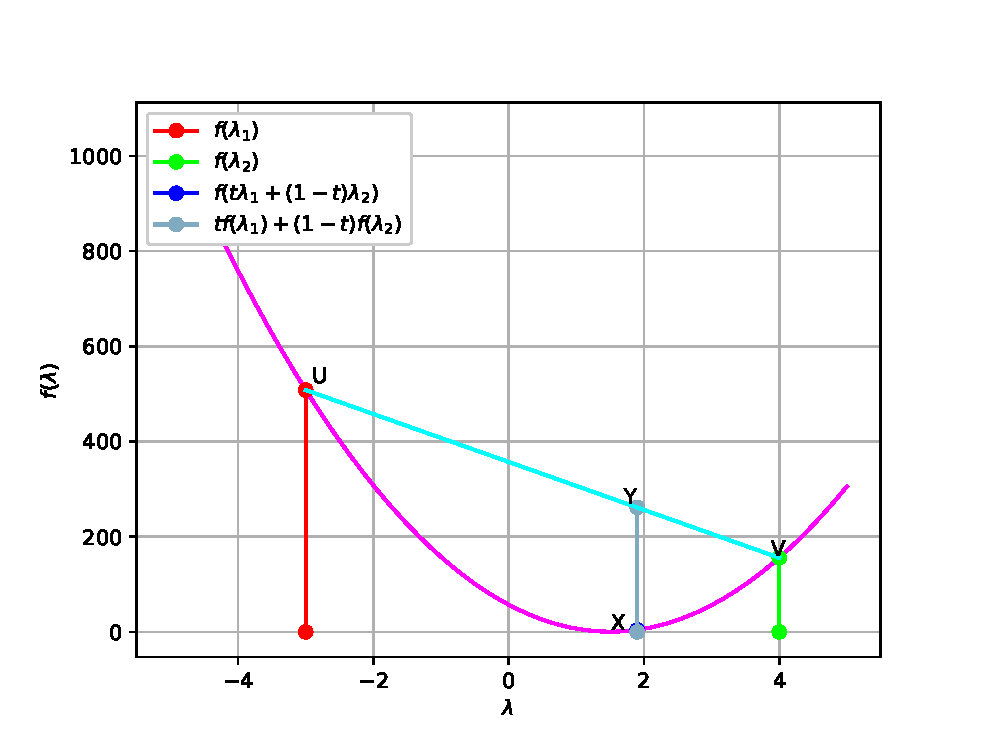
\includegraphics[width=\columnwidth]{./figs/convex.eps}
\caption{ $f(\lambda)$ versus $\lambda$}.
\label{fig:conv_def}	
\end{figure}
%
\item Show that
%
\begin{align}
\label{eq:convex_def}
f\sbrak{t \lambda_1 + \brak{1-t}\lambda_2} \leq 
t f\brak{\lambda_1} + \brak{1-t}f\brak{\lambda_2}
\end{align}
%
for $\quad 0 < t < 1$.  This is true for any convex function.
%
\item Show that 
%
\begin{equation}
\eqref{eq:convex_def} \quad \implies f^{(2)}(\lambda) > 0
\end{equation}
%
\item Show that a covex function has a unique minimum.
%
\end{enumerate}
%

%\section{Gradient Descent}
%\renewcommand{\theequation}{\theenumi}
\begin{enumerate}[label=\arabic*.,ref=\thesection.\theenumi]
\numberwithin{equation}{enumi}
%\item Consider the problem of finding the square root of a number $c$.  This can be expressed as the equation
%%
%\begin{equation}
%\label{eq:root}
%x^2 -c= 0
%\end{equation}
%%
%
%\item
%Sketch the function for different values of $c$
%%
%\begin{equation}
%f(x)= x^{3}-3xc
%\end{equation}
%%
%and comment upon its convexity.
%
%\item
%Show that \eqref{eq:root} results from
%\begin{align}
%\min_{x}f(x)= x^{3}-3xc
%\end{align}

\item
Find a numerical solution for \eqref{eq:parab}

%
%\begin{align}
%f(\lambda) = a\lambda^2 + b\lambda + d
%\end{align}
%
%\eqref{eq:root}.
%\\
\solution
A numerical solution for \eqref{eq:root} is obtained as
%
\begin{align}
\lambda_{n+1}&=\lambda_{n}-\mu f^{\prime}\brak{\lambda_n}
\\
&=\lambda_{n} -\mu \brak{2a\lambda_n+b}
\label{eq:gradient}
\end{align}

%\begin{align}
%x_{n+1}&=x_{n}-{\frac {f(x_{n})}{f^{\prime}(x_{n})}}
%\\
%&=x_{n} -\frac{x^2_{n}-c}{2x_n} 
%\\
%&=\frac{1}{2}\sbrak{x_{n} +\frac{c}{x_n} }
%\label{eq:newton}
%\end{align}
%
where $\lambda_0$ is an inital guess.
%
\item
Write a program to implement \eqref{eq:gradient}.
%
\\
\solution Download and execute
\begin{lstlisting}
codes/optimization/gd.py
\end{lstlisting}
%
\item Find a closed form solution for \eqref{eq:gradient} using the one sided Z transform.
%
\item Find the condition for which \eqref{eq:gradient} converges, i.e.
\begin{align}
\lim_{n \to \infty}\abs{\lambda_{n+1}-\lambda_n} = 0
\end{align}
\end{enumerate}


%\section{Lagrange Multipliers}
%\renewcommand{\theequation}{\theenumi}
\begin{enumerate}[label=\arabic*.,ref=\thesection.\theenumi]
\numberwithin{equation}{enumi}

\item
	\label{convex_code}
Find
\begin{align}
\label{eq:opt_line_nor_h}
	\min_{\mbf{x}}g\brak{\mbf{x}} = \norm{\vec{x}-\vec{P}}^2 = r^2 \\
\text{s.t.} \quad 	h\brak{\mbf{x}} = \vec{n}^T\vec{x} - c = 0\label{eq2_1_line}
%	\quad g\brak{\mbf{x}} = x_1 + x_2 - 9 = 0
\end{align}
by plotting the circles $g\brak{\vec{x}}$
%
%\begin{equation}
% \norm{\vec{x}-\myvec{8\\6}}^2 =r^2
%%(x_1-8)^2 + (x_2-6)^2 = r^2
%\end{equation}
%
% $\mbf{x}= \myvec{x_1\\x_2}$, 
for different values of $r$ along with the line $g\brak{\mbf{x}}$.
%
%\begin{equation}
%\label{eq2_1_line}
%g\brak{\mbf{x}} = \myvec{1 & 1}\vec{x} - 9 = 0
%\end{equation} 
%
\\
\solution 
The following code plots Fig. \ref{fig.concirc}	

%	
\begin{lstlisting}
codes/optimization/concirc.py
\end{lstlisting}

%
\begin{figure}[!ht]
\centering
\includegraphics[width=\columnwidth]{./figs/concirc.eps}
\caption{ Finding $ \displaystyle \min_{\mbf{x}}g\brak{\mbf{x}}$}.
\label{fig.concirc}	
\end{figure}
%
\item By solving the quadratic equation obtained from \eqref{eq:opt_line_nor_h},
show that 
\label{prob:minr}
\begin{align}
\min_{\vec{x}} r = \frac{3}{5}
\end{align}
%
and find $\vec{x} = \vec{Q}$ that minimizes $r$. By labeling  $\vec{Q}$ in Fig. \ref{fig:concirc}, show that $\vec{Q}$ is the point of contact of the line $L$ with the circle of minimum radius $r = \frac{3}{5}$.
%Obtain a theoretical solution for problem \ref{convex_code} 
%%using coordinate geometry.
%
%\solution 
%From \eqref{eq2_1_line} and \eqref{eq2_1_circ}, 
%%
%\begin{align}
%r^2 & = (x_1-8)^2 + (3- x_1)^2 \\
%&= 2 x_1^2 - 22 x_1 + 73 \\
%\Rightarrow r^2 &= \frac{\brak{2x_1-11}^2 + 5^2}{2}
%\end{align}
%%
%which is minium when $x_1 = \frac{11}{2}, x_2 = \frac{7}{2}$.  The minimum value is $\frac{25}{2}$ and 
%the radius $r = \frac{5}{\sqrt{2}}$.
\item Show that 
\begin{align}
\nabla h(\vec{x}) =  \myvec{3 \\ -4} = \vec{n}
\end{align}
where
\begin{equation}
\nabla =  
\begin{pmatrix}
\frac{\partial}{\partial x_1} \\
\frac{\partial}{\partial x_2} 
\end{pmatrix}
\end{equation}

\item Show that 
\begin{align}
\nabla g(\vec{x}) = 2\cbrak{\vec{x}-\myvec{3 \\ -5}} = 2\cbrak{\vec{x}-\vec{P}}
\end{align}
%
%is the direction vector of the normal at $\vec{x}$.
\item From Fig. \ref{fig.concirc}, show that 
\begin{align}
\label{eq:opt_normal}
\nabla g(\vec{Q}) = \lambda \nabla h(\vec{Q}),
\end{align}
%
%where $\vec{p}$ is the point of contact.
\item Use \eqref{eq:opt_normal} and $\vec{h(\vec{Q})}=0$ from \eqref{eq2_1_line} to obtain $\vec{Q}$.
\item
\label{lagrange}
	Define 
	\begin{equation}
	\label{lagrangian}
	C\brak{\mbf{x},\lambda} = g\brak{\mbf{x}} - \lambda h\brak{\mbf{x}}%, \quad \lambda > 0
	\end{equation}
and show that $\vec{Q}$ can also be obtained by 
solving the equations
%
\begin{align}
\nabla C\brak{\mbf{x},\lambda} &= 0.
\label{tangent}
\end{align}
%
What is the sign of $\lambda$?  $C$ is known as the Lagrangian and the above technique is known as the Method of Lagrange Multipliers.

\solution
%From \eqref{eq2_1_line} and \eqref{eq2_1_circ}, 
%%
%\begin{align}
%L\brak{\mbf{x},\lambda} &= (x_1-8)^2 + (x_2-6)^2 - \lambda \brak{x_1 + x_2 - 9} \\
%\Rightarrow \nabla L\brak{\mbf{x},\lambda}  & = 
%\begin{pmatrix}
%2x_1  - 16 - \lambda \\
%2x_2 - 12 - \lambda \\
%x_1 + x_2 -9
%\end{pmatrix}
%\\
%&=
%\begin{pmatrix}
%2 &0 & - 1 \\
%0 &2 & - 1 \\
%1 & 1 & 0 
%\end{pmatrix}
%\begin{pmatrix}
%x_1 \\
%x_2 \\
%\lambda
%\end{pmatrix}
%= 
%\begin{pmatrix}
%16 \\
% 12 \\
%9
%\end{pmatrix}
%=
%0 
%\\
%\Rightarrow 
%\begin{pmatrix}
%x_1 \\
%x_2 \\
%\lambda
%\end{pmatrix}
%&= 
%\begin{pmatrix}
%\frac{11}{2} \\
% \frac{7}{2} \\
%-5
%\end{pmatrix}
%\end{align}
%%
%using the following python script.  Note that this method yields the same result as the previous exercises.  Thus, $\lambda$ is negative.
%	
\begin{lstlisting}
codes/optimization/lagmul.py
\end{lstlisting}
\item Obtain $\vec{Q}$ using gradient descent.
\end{enumerate}

%\section{Quadratic Programming}
%\renewcommand{\theequation}{\theenumi}
\begin{enumerate}[label=\arabic*.,ref=\thesection.\theenumi]
\numberwithin{equation}{enumi}

\item An apache helicopter of the enemy is flying along the curve given by 
	\label{prob:dist_pt_parab}
\begin{align}
\label{eq:dist_pt_parab}
y = x^2 +7
\end{align}
%
A soldier, placed at 
\begin{align}
\vec{P} = \myvec{3\\7}.  
\end{align}
%
wants to shoot the heicopter when it is nearest to him.  Express this as an optimization problem.
%\item
%Express the problem of 
%finding the point on the curve 
%\begin{align}
%\label{eq:dist_pt_parab}
%x^2 = 2y
%\end{align}
%%
%nearest to the point 
%\begin{align}
%\vec{P} = \myvec{0\\5}.  
%\end{align}
%%
%as an optiimization problem.
\\
\solution The given problem can be expressed as
\begin{align}
\label{eq:qp_dist_pt_parab}
\min_{\vec{x}}\norm{\vec{x}-\vec{P}}^2
\\
\text{s.t. }\vec{x}^T\vec{V}\vec{x} + \vec{u}^T\vec{x}  +d = 0
\end{align}
%
where
%
\begin{align}
\vec{V} &= \myvec{1 & 0\\0 & 0}
\\
\vec{u} &= -\myvec{0 \\ 1}
\\
d &= 7
\end{align}
\item Show that the constraint in \ref{eq:qp_dist_pt_parab} is nonconvex.
\item Show that the following {\em relaxation} makes \eqref{eq:qp_dist_pt_parab} a convex optimization problem.
%
\begin{align}
\label{eq:qp_dist_pt_parab_conv}
\min_{\vec{x}}\brak{\vec{x}-\vec{P}}^T\brak{\vec{x}-\vec{P}}
\\
\text{s.t. }\vec{x}^T\vec{V}\vec{x} + \vec{u}^T\vec{x}  \le 0
\end{align}
%
%
\item Solve \eqref{eq:qp_dist_pt_parab_conv} using cvxpy.
\\
\solution  The following code yields the minimum distance as 2.236 and the nearest point on the curve as
%
\begin{align}
\vec{Q} &= \myvec{1\\8}
\end{align}

\begin{lstlisting}
codes/qp_cvx.py
\end{lstlisting}

\item Solve \eqref{eq:qp_dist_pt_parab_conv} using the method of Lagrange multipliers.
\item Graphically verify the solution to Problem \ref{prob:dist_pt_parab}. 
%by drawing a figure.
\\
\solution 
The following code plots Fig. \label{fig:qp_parab}
%	
\begin{lstlisting}
codes/qp_parab.py
\end{lstlisting}

%
\begin{figure}[!ht]
\centering
\includegraphics[width=\columnwidth]{./figs/qp_parab.eps}
\caption{ $\vec{Q}$ is closest to $\vec{P}$}.
\label{fig:qp_parab}
\end{figure}
%
%\item Frame 	
% as an optimization problem.
%\label{prob:qp_dist_pt_parab}
%\\
%
%\solution 
%From \eqref{eq2_1_line} and \eqref{eq2_1_circ}, 
%%
%\begin{align}
%r^2 & = (x_1-8)^2 + (3- x_1)^2 \\
%&= 2 x_1^2 - 22 x_1 + 73 \\
%\Rightarrow r^2 &= \frac{\brak{2x_1-11}^2 + 5^2}{2}
%\end{align}
%%
%which is minium when $x_1 = \frac{11}{2}, x_2 = \frac{7}{2}$.  The minimum value is $\frac{25}{2}$ and 
%the radius $r = \frac{5}{\sqrt{2}}$.
%	
%\begin{lstlisting}
%codes/optimization/lagmul.py
%\end{lstlisting}
\item Solve \eqref{eq:qp_dist_pt_parab_conv} using gradient descent.
%
\end{enumerate}

%\section{Semi Definite Programming}
%\renewcommand{\theequation}{\theenumi}
\begin{enumerate}[label=\arabic*.,ref=\thesection.\theenumi]
\numberwithin{equation}{enumi}

%\item An apache helicopter of the enemy is flying along the curve given by 
%	\label{prob:dist_pt_parab_sdp}
%\begin{align}
%\label{eq:dist_pt_parab_sdp}
%y = x^2 +7
%\end{align}
%%
%A soldier, placed at 
%\begin{align}
%\vec{P} = \myvec{3\\7}.  
%\end{align}
%%
%wants to shoot the heicopter when it is nearest to him.  Express this as an optimization problem.
\item
	\label{prob:dist_pt_parab_sdp}
Express the problem of 
finding the point on the curve 
\begin{align}
\label{eq:dist_pt_parab_sdp}
x^2 = 2y
\end{align}
%
nearest to the point 
\begin{align}
\vec{P} = \myvec{0\\5}.  
\end{align}
%
as an optimization problem.
\\
\solution The given problem can be expressed as
%
\begin{align}
\label{eq:qp_dist_pt_parab_sdp_qp}
\min_{\vec{x}}\vec{x}^T\vec{Q}_0\vec{x}+\vec{q}_0^T\vec{x}+c_0
\\
\text{s.t. }\vec{x}^T\vec{Q}_1\vec{x} + \vec{q}_1^T\vec{x} +c_1 \le 0
\end{align}
%
%where $\vec{V} \succeq 0$.
%\begin{align}
%\label{eq:qp_dist_pt_parab_sdp}
%\begin{split}
%\min_{\vec{x}}\vec{X}^T\myvec{\vec{I} & \vec{0} \\ \vec{0} & \vec{0}}\vec{X}-2\myvec{\vec{P}^T & \vec{0}}\vec{X}+\norm{\vec{P}}^2
%\\
%\text{s.t. }\vec{x}^T\vec{V}\vec{x} + \vec{u}^T\vec{x}  = 0
%\end{split}
%\end{align}
%
where
%
\begin{align}
\vec{Q}_0 &= \vec{I}, \vec{Q}_1 = \myvec{1 & 0\\0 & 0}
\\
\vec{q}_0 &=-2\vec{P}, \vec{q}_1 = -2\myvec{0 \\ 1}
\\
c_0 &= \norm{\vec{P}}^2, c_1 = 0
\end{align}
%\item Show that the constraint in 	
%%\label{prob:dist_pt_parab_sdp}
%\eqref{eq:qp_dist_pt_parab_sdp} is nonconvex.
%
\item Show that \eqref{eq:qp_dist_pt_parab_sdp_qp} is equivalent to
\begin{align}
\label{eq:qp_dist_pt_parab_sdp_conv}
\begin{split}
\min_{\vec{x},\theta}\theta
\\
\text{s.t. } \myvec{\vec{I} & \vec{M}_0\vec{x} \\ \vec{x}^T\vec{M}_0^T & -c_0-q_0^T\vec{x}+\theta} &\succeq 0
\\
\myvec{\vec{I} & \vec{M}_1\vec{x} \\ \vec{x}^T\vec{M}_1^T & -c_1-q_1^T\vec{x}} &\succeq 0
\end{split}
\end{align}
%
%\item Show that the following {\em relaxation} makes \eqref{eq:qp_dist_pt_parab_sdp} a convex optimization problem.
%%
%\begin{align}
%\label{eq:qp_dist_pt_parab_sdp_conv}
%\min_{\vec{x}}\brak{\vec{x}-\vec{P}}^T\brak{\vec{x}-\vec{P}}
%\\
%\text{s.t. }\vec{x}^T\vec{V}\vec{x} + \vec{u}^T\vec{x}  \le 0
%\end{align}
%
where
\begin{align}
\vec{Q}_i = \vec{M}_i^T\vec{M}_i, i = 0, 1
\end{align}
%
\item Solve \eqref{eq:qp_dist_pt_parab_sdp_conv} using cvxpy.
\item Graphically verify the solution to Problem \ref{prob:dist_pt_parab_sdp}. 
%\\
%\solution  The following code yields the minimum distance as 2.236 and the nearest point on the curve as
%%
%\begin{align}
%\vec{Q} &= \myvec{1\\8}
%\end{align}
%
%\begin{lstlisting}
%codes/qp_cvx.py
%\end{lstlisting}

\item Solve \eqref{eq:qp_dist_pt_parab_sdp_qp} using the method of Lagrange multipliers.
%by drawing a figure.
%\\
%\solution 
%The following code plots Fig. \label{fig:qp_parab_sdp}
%%	
%\begin{lstlisting}
%codes/qp_parab.py
%\end{lstlisting}
%
%%
%\begin{figure}[!ht]
%\centering
%\includegraphics[width=\columnwidth]{./figs/qp_parab.eps}
%\caption{ $\vec{Q}$ is closest to $\vec{P}$}.
%\label{fig:qp_parab_sdp}
%\end{figure}
%
%\item Frame 	
% as an optimization problem.
%\label{prob:qp_dist_pt_parab}
%\\
%
%\solution 
%From \eqref{eq2_1_line} and \eqref{eq2_1_circ}, 
%%
%\begin{align}
%r^2 & = (x_1-8)^2 + (3- x_1)^2 \\
%&= 2 x_1^2 - 22 x_1 + 73 \\
%\Rightarrow r^2 &= \frac{\brak{2x_1-11}^2 + 5^2}{2}
%\end{align}
%%
%which is minium when $x_1 = \frac{11}{2}, x_2 = \frac{7}{2}$.  The minimum value is $\frac{25}{2}$ and 
%the radius $r = \frac{5}{\sqrt{2}}$.
%	
%\begin{lstlisting}
%codes/optimization/lagmul.py
%\end{lstlisting}
%\item Solve \eqref{eq:qp_dist_pt_parab_sdp_conv} using gradient descent.
%
\end{enumerate}

%\section{Linear Programming}
%\renewcommand{\theequation}{\theenumi}
\begin{enumerate}[label=\arabic*.,ref=\thesection.\theenumi]
\numberwithin{equation}{enumi}
%
\item Solve
\label{prob:lp_std}
\begin{align}
\max_{\vec{x}} Z &= \myvec{4 & 1}\vec{x}
\\
s.t. \quad 
\myvec{
1 & 1
\\
3 & 1
}
\vec{x} &\preceq \myvec{50\\90}
\\
\vec{x} &\succeq \vec{0}
\end{align}
%
using cvxpy.
\\
\solution The given problem can be expressed in general as
\begin{align}
\max_{\vec{x}} &\vec{c}^{T}\vec{x}
\\
s.t. \quad \vec{A}\vec{x} &\le \vec{b},
\\
\vec{x} &\succeq\vec{0}
\end{align}
%
where
\begin{align}
\vec{c} &= \myvec{4 \\ 1}
\\
\vec{A} &=
\myvec{
1 & 1
\\
3 & 1
}
\\
\vec{b}&=\myvec{50\\90}
%
\end{align}
%
and can be solved using {\em cvxpy} through the following code
\begin{lstlisting}
codes/lp_cvx.py
\end{lstlisting}
%
to obtain
\begin{align}
\vec{x} = \myvec{30\\0}, Z = 120
\end{align}
%
\item Graphically, show that the {feasible region} in  Problem \ref{prob:lp_std} result in the interior of a convex polygon and the optimal point is one of the vertices.
\solution The following code plots Fig. \ref{fig:lp_feas_reg}.
%
\begin{lstlisting}
codes/lp_cvx.py
\end{lstlisting}
%
\begin{figure}[!ht]
\includegraphics[width=\columnwidth]{./figs/lp_feas_reg.eps}
\caption{}
\label{fig:lp_feas_reg}
\end{figure}

%Verify the solution to graphically.
\item Solve
\begin{align}
\min_{\vec{x}} Z &= \myvec{3 & 9}\vec{x}
\\
s.t. \quad 
\myvec{
1 & 3
\\
-1 & -1
\\
1 & -1
}
\vec{x} &\preceq \myvec{60\\-10\\0}
\\
\vec{x} &\succeq \vec{0}
\label{eq:lp_exam_mult}
\end{align}
\solution The following code
\begin{lstlisting}
codes/lp_cvx_mult.py
\end{lstlisting}
%
is used to obtain
\begin{align}
\vec{x} = \myvec{15\\15}, Z = 180
\end{align}
%
%\item Write a program to plot the constraints for any linear program.

%The region in \eqref{eq:lp_constr} is shown in Fig. \ref{}
\item Solve
\begin{align}
\min_{\vec{x}} Z &= \myvec{-50 & 20}\vec{x}
\\
s.t. \quad 
\myvec{
-2 & 1
\\
-3 & -1
\\
2 & -3
}
\vec{x} &\preceq \myvec{5\\-3\\12}
\\
\vec{x} &\succeq \vec{0}
\end{align}
%
\solution The following code 
\begin{lstlisting}
codes/lp_cvx_nosol.py
\end{lstlisting}
%
shows that the given problem has no solution.
\item Verify all the above solutions using Lagrange multipliers.
\item Repeat the above exercise using the Simplex method.
\item\textbf {(Diet problem)}: A dietician wishes to mix two types of foods in such a
way that vitamin contents of the mixture contain atleast 8 units of vitamin A and 10
units of vitamin C. Food ‘I’ contains 2 units/kg of vitamin A and 1 unit/kg of vitamin C.
Food ‘II’ contains 1 unit/kg of vitamin A and 2 units/kg of vitamin C. It costs
Rs 50 per kg to purchase Food ‘I’ and Rs 70 per kg to purchase Food ‘II’. Formulate
this problem as a linear programming problem to minimise the cost of such a mixture.
\\
\solution Let the mixture contain $x$ kg of food I and $y$ kg of food II.
\\
\begin{table}[!h]
\begin{tabular}{|l|l|l|l|}
\hline
\multirow{2}{*}{Resources} & \multicolumn{2}{l|}{Food} & \multirow{2}{*}{Requirement} \\ \cline{2-3}
                           & I           & II          &                              \\ \hline
Vitamin A                  & 2           & 1           & Atleast 8 Units              \\ \hline
Vitamin C                  & 1           & 2           & Atleast 10 Units             \\ \hline
Cost                       & 50          & 70          &                              \\ \hline
\end{tabular}
\end{table}
%
The given problem can be expressed as
%GOAL: We need to minimize the cost of mixture.\\
%Cost of FOOD I per kg = Rs 50 \\
%Cost of FOOD II per kg = Rs 70 \\
% Minimize $ Z = 50x +70y$\\
% Subject to constraints:\\
% $2x+y>=8$\\
% $x+2y>=10$\\
% $x,y>=0$\\
\begin{align}
\min_{\vec{x}} Z &= \myvec{50 & 70}\vec{x}
\\
s.t. \quad 
\myvec{
2 & 1
\\
1 & 2
%\\
%2 & -3
}
\vec{x} & \succeq \myvec{8\\10}
%\preceq \myvec{5\\-3\\12}
\\
\vec{x} &\succeq \vec{0}
\label{eq:diet}
\end{align}
%
The corner points of the feasible region are available in Table \ref{table:diet_corner_pt} and plotted in Fig. \ref{fig:diet}.
%
\begin{table}[!h]
\begin{tabular}{|l|l|l|l|}
\hline
Corner Point &  $Z=50x+70y$\\
\hline
(0,8)& 560\\
\hline
(2,4)& 380\\
\hline
(10,0)& 500\\
\hline
\end{tabular}
\caption{}
\label{table:diet_corner_pt}
\end{table}
  \begin{figure}[!h]

  \centering
  \includegraphics[width=1\linewidth]{./figs/lp_diet.eps}
\caption{}
\label{fig:diet}
  \end{figure}


The smallest value of Z is 380 at the point (2,4). But the feasible region is unbounded therefore we draw the graph of the inequality
\begin{align}
50x +70y<380
\end{align}
to check whether the resulting open half has any point common with the feasible region but on checking it doesn't have any points in common. 
Thus the minimum value of Z is 380 attained at $\myvec{2\\4}$. Hence optimal mixing strategy for the dietician would be to mix 2 Kg of Food I and 4 Kg of Food II.  The following code provides the solution to \eqref{eq:diet}.
%
\begin{lstlisting}
codes/diet.py
\end{lstlisting}



\item \textbf{(Allocation problem)} A cooperative society of farmers has 50 hectare
of land to grow two crops X and Y. The profit from crops X and Y per hectare are
estimated as Rs 10,500 and Rs 9,000 respectively. To control weeds, a liquid herbicide
has to be used for crops X and Y at rates of 20 litres and 10 litres per hectare. Further,
no more than 800 litres of herbicide should be used in order to protect fish and wild life
using a pond which collects drainage from this land. How much land should be allocated
to each crop so as to maximise the total profit of the society?\\
\solution The given problem can be formulated as
\begin{align}
\max_{\vec{x}} Z &= \myvec{10500 & 9000}\vec{x}
\\
s.t. \quad 
\myvec{
20 & 10
}
\vec{x} & \preceq 800
\\
\myvec{
1 & 1
} 
\vec{x} &= 50
\label{eq:allocation}
\end{align}
Fig  \ref{fig:allocation}
shows the intersection of various lines and the optimal point as indicated.
%\begin{figure}[h]
%\includegraphics[width=\columnwidth]{./figs/lp_allocation.eps}
%\caption{Feasible region for allocation Problem}
%\caption{}
%\label{fig:allocation}
%\end{figure}

The following code provides the solution to \eqref{eq:allocation} at \myvec{12\\6}.
%
\begin{lstlisting}
codes/allocation.py
\end{lstlisting}

\item  \textbf{(Manufacturing problem)} A manufacturing company makes two models
A and B of a product. Each piece of Model A requires 9 labour hours for fabricating
and 1 labour hour for finishing. Each piece of Model B requires 12 labour hours for
fabricating and 3 labour hours for finishing. For fabricating and finishing, the maximum
labour hours available are 180 and 30 respectively. The company makes a profit of
Rs 8000 on each piece of model A and Rs 12000 on each piece of Model B. How many
pieces of Model A and Model B should be manufactured per week to realise a maximum
profit? What is the maximum profit per week?\\
\item \textbf {(Diet problem)} A dietician has to develop a special diet using two foods
P and Q. Each packet (containing 30 g) of food P contains 12 units of calcium, 4 units
of iron, 6 units of cholesterol and 6 units of vitamin A. Each packet of the same quantity
of food Q contains 3 units of calcium, 20 units of iron, 4 units of cholesterol and 3 units
of vitamin A. The diet requires atleast 240 units of calcium, atleast 460 units of iron and
at most 300 units of cholesterol. How many packets of each food should be used to
minimise the amount of vitamin A in the diet? What is the minimum amount of vitamin A?\\
\item \textbf{(Manufacturing problem)} A manufacturer has three machines I, II
and III installed in his factory. Machines I and II are capable of being operated for
at most 12 hours whereas machine III must be operated for atleast 5 hours a day. She
produces only two items M and N each requiring the use of all the three machines.
The number of hours required for producing 1 unit of each of M and N on the three
machines are given in the following table:\\

\begin{tabular}{|c|c|c|c|}
\hline
 \multicolumn{3}{|l}{\textbf{ Number of hours required on machines}}& \\ \cline{2-4}
\hline
\textbf {Items}&\textbf{I}&\textbf{II}&\textbf{III}\\
\hline
M&1&2&1\\
\hline
 N&2&1&1.25\\
 \hline 

\end{tabular}

She makes a profit of Rs 600 and Rs 400 on items M and N respectively. How many
of each item should she produce so as to maximise her profit assuming that she can sell
all the items that she produced? What will be the maximum profit?
\\
\solution The given problem can be formulated as
\begin{align}
\max_{\vec{x}} Z &= \myvec{80000&12000}\vec{x}
\\
s.t. \quad 
\myvec{
3 & 4
\\
1 & 3
}
\vec{x} & \preceq \myvec{60\\30}
\label{eq:manufacturing}
\end{align}

Fig  \ref{fig:manufacturing}
shows the intersection of various lines and the optimal point as indicated.
\begin{figure}[h]
\includegraphics[width=\columnwidth]{./figs/lp_manufacturing.eps}
\caption{Feasible region for manufacturing Problem}
\caption{}
\label{fig:manufacturing}
\end{figure}

The following code provides the solution to \eqref{eq:manufacturing} at \myvec{12\\6}.
%
\begin{lstlisting}
codes/Manufacturing.py
\end{lstlisting}

\item \textbf{(Transportation problem)} There are two factories located one at
place P and the other at place Q. From these locations, a certain commodity is to be
delivered to each of the three depots situated at A, B and C. The weekly requirements
of the depots are respectively 5, 5 and 4 units of the commodity while the production
capacity of the factories at P and Q are respectively 8 and 6 units. The cost of transportation per unit is given below where A,B,C are cost in ruppes:\\
\begin{tabular}{|c|c|c|c|}
\hline
From/To & A & B & C\\
\hline
P & 160 & 100 & 150\\
\hline
Q & 100 &120 & 100\\
\hline
\end{tabular}\\
How many units should be transported from each factory to each depot in order that
the transportation cost is minimum. What will be the minimum transportation cost?
\\
\solution The given problem can be formulated as
\begin{align}
\min_{\vec{x}} Z &= \myvec{10 & -70}\vec{x}
\\
s.t. \quad 
\myvec{
1 & 1
\\
-1 & -1
}
\vec{x} & \preceq \myvec{8\\-4}
\\
\vec{x} &\preceq \myvec{5\\5}
\label{eq:transport}
\end{align}

Fig  \ref{fig:transport}
shows the intersection of various lines and the optimal point indicated as OPT PT.
\begin{figure}[h]
\includegraphics[width=\columnwidth]{./figs/lp_transport.eps}
\caption{Feasible region for Transportation Problem}
\caption{}
\label{fig:transport}
\end{figure}

The following code provides the solution to \eqref{eq:transport} at \myvec{0\\5}.
%
\begin{lstlisting}
codes/Transportation.py
\end{lstlisting}





\end{enumerate}
%    \end{document}
    

%\section{Exercises}
%\renewcommand{\theequation}{\theenumi}
\begin{enumerate}[label=\arabic*.,ref=\thesubsection.\theenumi]
\numberwithin{equation}{enumi}

\item Solve
\begin{align}
\min_{\vec{x}} Z &= \myvec{3 & 2}\vec{x}
\\
s.t. \quad 
\myvec{
-1 & -1
\\
3 & 5
}
\vec{x} &\preceq \myvec{-8\\15}
\\
\vec{x} &\succeq \vec{0}
\end{align}
\item Solve
\begin{align}
\min_{\vec{x}} Z &= \myvec{200 & 500}\vec{x}
\\
s.t. \quad 
\myvec{
-1 & -2
\\
3 & 4
}
\vec{x} &\preceq \myvec{-10\\24}
\\
\vec{x} &\succeq \vec{0}
\end{align}
\item Maximise Z=3x+4y\\
subject to the constraints : x+y$\leq$4, x$\geq$0, y$\geq$ 0.\\
\item Minimise Z=-3x+4y\\
subject to x+2y$\leq$8, 3x+2y$\leq$12, x$\geq$0, y$\geq$0.\\
\item Maximise Z=5x+3y
subject to 3x+5y$\leq$15, 5x+2y$\leq$10, x$\geq$0, y$\geq$0.\\
\item Minimise Z=3x+5y
such that x+3y$\geq$3, x+y$\geq$2, x,y$\geq$0.\\
\item Maximise Z=3x+2y
subject to x+2y$\leq$10, 3x+y$\leq$15, x,y$\geq$0.\\
\item Minimise Z=x+2y
subject to 2x+y$\geq$3, x+2y$\geq$6, x,y$\geq$0.\\
Show that the minimum of Z occurs at more than two points.\\
\item Minimise and Maximise Z=5x+10y
subject to x+2y$\leq$120, x+y$\geq$60, x-2y$\geq$0, x,y$\geq$0.\\
\item Minimise and Maximise Z=x+2y
subject to x+2y$\geq$100, 2x-y$\leq$0, 2x+y$\leq$200; x,y$\geq$0.\\
\item Maximise Z=-x+2y, subject to the constraints:
x$\geq$3, x+y$\geq$5, x+2y$\geq$6, y$\geq$0.\\
\item Maximise Z=x+y, subject to x-y$\leq$-1,-x+y$\leq$0, x,y$\geq$0.\\
\item Reshma wishes to mix two types of food P and Q in such a way that the vitamin
contents of the mixture contain at least 8 units of vitamin A and 11 units of
vitamin B. Food P costs Rs 60/kg and Food Q costs Rs 80/kg. Food P contains
3 units/kg of Vitamin A and 5 units/kg of Vitamin B while food Q contains
4 units/kg of Vitamin A and 2 units/kg of vitamin B. Determine the minimum cost
of the mixture.\\
\item One kind of cake requires 200g of flour and 25g of fat, and another kind of cake
requires 100g of flour and 50g of fat. Find the maximum number of cakes which
can be made from 5kg of flour and 1 kg of fat assuming that there is no shortage
of the other ingredients used in making the cakes.\\
\item A factory makes tennis rackets and cricket bats. A tennis racket takes 1.5 hours
of machine time and 3 hours of craftman’s time in its making while a cricket bat
takes 3 hour of machine time and 1 hour of craftman’s time. In a day, the factory
has the availability of not more than 42 hours of machine time and 24 hours of
craftsman’s time.\\
(i) What number of rackets and bats must be made if the factory is to work
at full capacity?\\
(ii)If the profit on a racket and on a bat is Rs 20 and Rs 10 respectively, find
the maximum profit of the factory when it works at full capacity.\\
\item A manufacturer produces nuts and bolts. It takes 1 hour of work on machine A
and 3 hours on machine B to produce a package of nuts. It takes 3 hours on
machine A and 1 hour on machine B to produce a package of bolts. He earns a
profit of Rs17.50 per package on nuts and Rs 7.00 per package on bolts. How
many packages of each should be produced each day so as to maximise his
profit, if he operates his machines for at the most 12 hours a day?\\
\item A factory manufactures two types of screws, A and B. Each type of screw
requires the use of two machines, an automatic and a hand operated. It takes
4 minutes on the automatic and 6 minutes on hand operated machines to
manufacture a package of screws A, while it takes 6 minutes on automatic and
3 minutes on the hand operated machines to manufacture a package of screws
B. Each machine is available for at the most 4 hours on any day. The manufacturer
can sell a package of screws A at a profit of Rs 7 and screws B at a profit of
Rs 10. Assuming that he can sell all the screws he manufactures, how many
packages of each type should the factory owner produce in a day in order to
maximise his profit? Determine the maximum profit.\\
\item A cottage industry manufactures pedestal lamps and wooden shades, each
requiring the use of a grinding/cutting machine and a sprayer. It takes 2 hours on
grinding/cutting machine and 3 hours on the sprayer to manufacture a pedestal
lamp. It takes 1 hour on the grinding/cutting machine and 2 hours on the sprayer
to manufacture a shade. On any day, the sprayer is available for at the most 20
hours and the grinding/cutting machine for at the most 12 hours. The profit from
the sale of a lamp is Rs 5 and that from a shade is Rs 3. Assuming that the
manufacturer can sell all the lamps and shades that he produces, how should he
schedule his daily production in order to maximise his profit?\\
\item A company manufactures two types of novelty souvenirs made of plywood.
Souvenirs of type A require 5 minutes each for cutting and 10 minutes each for
assembling. Souvenirs of type B require 8 minutes each for cutting and 8 minutes
each for assembling. There are 3 hours 20 minutes available for cutting and 4
hours for assembling. The profit is Rs 5 each for type A and Rs 6 each for type
B souvenirs. How many souvenirs of each type should the company manufacture
in order to maximise the profit?\\
\item A merchant plans to sell two types of personal computers – a desktop model and
a portable model that will cost Rs 25000 and Rs 40000 respectively. He estimates
that the total monthly demand of computers will not exceed 250 units. Determine
the number of units of each type of computers which the merchant should stock
to get maximum profit if he does not want to invest more than Rs 70 lakhs and if
his profit on the desktop model is Rs 4500 and on portable model is Rs 5000.\\
\item A diet is to contain at least 80 units of vitamin A and 100 units of minerals. Two
foods$ F_{1}$ and $F_{2}$ are available. Food $F_{1}$ costs Rs 4 per unit food and $F_{2}$ costs
Rs 6 per unit. One unit of food $F_{1}$ contains 3 units of vitamin A and 4 units of
minerals. One unit of food $F_{2}$ contains 6 units of vitamin A and 3 units of minerals.
Formulate this as a linear programming problem. Find the minimum cost for diet
that consists of mixture of these two foods and also meets the minimal nutritional
requirements.\\
\item There are two types of fertilisers $F_{1}$ and $F_{2}$.$F_{1}$ consists of $10\%$ nitrogen and $6\%$
phosphoric acid and $F_{2}$ consists of $5\%$ nitrogen and $10\%$ phosphoric acid. After
testing the soil conditions, a farmer finds that she needs atleast 14 kg of nitrogen
and 14 kg of phosphoric acid for her crop. If $F_{1}$ costs Rs 6/kg and $F_{2}$ costs
Rs 5/kg, determine how much of each type of fertiliser should be used so that
nutrient requirements are met at a minimum cost. What is the minimum cost?\\
\item The corner points of the feasible region determined by the following system of
linear inequalities:
2x+y$\leq$10, x+3y$\leq$15, x,y$\geq$0 are (0,0), (5,0),(3,4) and (0,5).Let
Z=px+qy, where p,q$>$0.Condition on p and q so that the maximum of Z
occurs at both (3,4) and (0,5) is\\
(A) p = q\\
(B) p = 2q\\
(C) p = 3q\\
(D) q = 3p\\
\item Refer to Example 9. How many packets of each food should be used to maximise
the amount of vitamin A in the diet? What is the maximum amount of vitamin A
in the diet?\\
\item A farmer mixes two brands P and Q of cattle feed. Brand P, costing Rs 250 per
bag, contains 3 units of nutritional element A, 2.5 units of element B and 2 units
of element C. Brand Q costing Rs 200 per bag contains 1.5 units of nutritional
element A, 11.25 units of element B, and 3 units of element C. The minimum
requirements of nutrients A, B and C are 18 units, 45 units and 24 units respectively.
Determine the number of bags of each brand which should be mixed in order to
produce a mixture having a minimum cost per bag? What is the minimum cost of
the mixture per bag?\\
\item A dietician wishes to mix together two kinds of food X and Y in such a way that
the mixture contains at least 10 units of vitamin A, 12 units of vitamin B and
8 units of vitamin C. The vitamin contents of one kg food is given below:\\
\begin{tabular}{|c|c|c|c|}
\hline
\textbf{Food} &\textbf{Vitamin A} &\textbf{Vitamin B} & \textbf{VitaminC}\\
\hline
X & 1 & 2 & 3\\
\hline
Y &2 &2 &1\\
\hline


\end{tabular}\\
One kg of food X costs Rs 16 and one kg of food Y costs Rs 20. Find the least
cost of the mixture which will produce the required diet?\\
\item A manufacturer makes two types of toys A and B. Three machines are needed
for this purpose and the time (in minutes) required for each toy on the machines
is given below:\\
\begin{tabular}{|c|c|c|c|}
\hline
 \multicolumn{3}{|r}{\textbf{ Machines}}& \\ \cline{2-4}
\hline
\textbf {Types of toys}&\textbf{I}&\textbf{II}&\textbf{III}\\
\hline
A&12&18&6\\
\hline
 B&6&0&9\\
 \hline 

\end{tabular}



Each machine is available for a maximum of 6 hours per day. If the profit on
each toy of type A is Rs 7.50 and that on each toy of type B is Rs 5, show that 15
toys of type A and 30 of type B should be manufactured in a day to get maximum
profit.\\
\item An aeroplane can carry a maximum of 200 passengers. A profit of Rs 1000 is
made on each executive class ticket and a profit of Rs 600 is made on each
economy class ticket. The airline reserves at least 20 seats for executive class.
However, at least 4 times as many passengers prefer to travel by economy class
than by the executive class. Determine how many tickets of each type must be
sold in order to maximise the profit for the airline. What is the maximum profit?\\
\item Two godowns A and B have grain capacity of 100 quintals and 50 quintals
respectively. They supply to 3 ration shops, D, E and F whose requirements are
60, 50 and 40 quintals respectively. The cost of transportation per quintal from
the godowns to the shops are given in the following table:\\
\begin{tabular}{|c|c|c|}
\hline
 \multicolumn{2}{|l}{\textbf{ Transportation cost per qunital (in Rs)}}& \\ \cline{2-3}
\hline
\textbf {From/To}&\textbf{A}&\textbf{B}\\
\hline
D&6&4\\
\hline
 E&3&2\\
 \hline 
 F&2.50&3\\
 \hline

\end{tabular}\\


How should the supplies be transported in order that the transportation cost is
minimum? What is the minimum cost?\\
\item An oil company has two depots A and B with capacities of 7000 L and 4000 L
respectively. The company is to supply oil to three petrol pumps, D, E and F
whose requirements are 4500L, 3000L and 3500L respectively. The distances
(in km) between the depots and the petrol pumps is given in the following table:\\
\begin{tabular}{|c|c|c|}
\hline
 \multicolumn{2}{|l}{\textbf{Distance in (km.)}}& \\ \cline{2-3}
\hline
\textbf {From/To}&\textbf{A}&\textbf{B}\\
\hline
D&7&3\\
\hline
 E&6&4\\
 \hline 
 F&3&2\\
 \hline

\end{tabular}\\

Assuming that the transportation cost of 10 litres of oil is Re 1 per km, how
should the delivery be scheduled in order that the transportation cost is minimum?
What is the minimum cost?\\
\item A fruit grower can use two types of fertilizer in his garden, brand P and brand Q.
The amounts (in kg) of nitrogen, phosphoric acid, potash, and chlorine in a bag of
each brand are given in the table. Tests indicate that the garden needs at least
240 kg of phosphoric acid, at least 270 kg of potash and at most 310 kg of
chlorine.
If the grower wants to minimise the amount of nitrogen added to the garden,
how many bags of each brand should be used? What is the minimum amount of
nitrogen added in the garden?\\
\begin{tabular}{|c|c|c|}
\hline
 \multicolumn{2}{|r}{\textbf{ kg per bag}}& \\ \cline{1-3}
\hline
&\textbf{Brand P}&\textbf{Brand Q}\\
\hline
Nitrogen&3&3.5\\
\hline
Phospheric acid&1&2\\
\hline
Potash&3&1.5\\
\hline
Chlorine&1.5&2\\
\hline

\end{tabular}

\item Refer to Question 29. If the grower wants to maximise the amount of nitrogen
added to the garden, how many bags of each brand should be added? What is
the maximum amount of nitrogen added?\\
\item A toy company manufactures two types of dolls, A and B. Market research and
available resources have indicated that the combined production level should not
exceed 1200 dolls per week and the demand for dolls of type B is at most half of that
for dolls of type A. Further, the production level of dolls of type A can exceed three
times the production of dolls of other type by at most 600 units. If the company
makes profit of Rs 12 and Rs 16 per doll respectively on dolls A and B, how many of
each should be produced weekly in order to maximise the profit?
\item Find the shortest distance of the point $\myvec{0\\c}$ from the parabola $y = x^2$, where $\frac{1}{2} \le c \le 5$.
\item Find the maximum area of an isosceles triangle inscribed in the ellipse 
%
\begin{align}
\vec{x}^T\myvec{a^2 & 0 \\ 0 & b^2}\vec{x} = a^2b^2
\end{align}
%
with its vertex at one end of the major axis.





\end{enumerate}
%\end{document}



\end{document}


